\def\mlnotes{}
\ifx\notes\undefined
    \providecommand{\notesroot}{..}
    \providecommand{\mlroot}{.}

    \title{机器学习}
    \author{Donald Cheung\\jianzhang9102@gmail.com}
    \date{\today\footnote{文档编写开始于2017年06月16日}}

    \documentclass[a4paper,10pt]{ctexbook}
\usepackage{xeCJK}
\usepackage{fontspec}
\usepackage{minted}
\usepackage[CJKbookmarks,colorlinks,linkcolor=red]{hyperref}
\usepackage{geometry}
\usepackage{amsmath}
\usepackage[format=hang,font=small,textfont=it]{caption}
\usepackage{float}
\usepackage{subfigure}
\usepackage[nottoc]{tocbibind}
\usepackage{bm}
\usepackage[table, x11names, dvipsnames]{xcolor}
\usepackage{color}
\usepackage{array, booktabs, boldline}
\usepackage{cellspace}
\usepackage{longtable}

\setmainfont{Times New Roman}
\setsansfont{Helvetica}
\setmonofont{Courier New}
\setCJKmainfont[BoldFont={SimHei},ItalicFont={SimHei}]{SimSun}
\setCJKsansfont{SimSun}
\setCJKmonofont{SimSun}

\setcounter{secnumdepth}{4}
\setcounter{tocdepth}{4}

\geometry{left=3.0cm,right=3.0cm,top=2.5cm,bottom=2.5cm}
\bibliographystyle{plain}

%%%%%%%%%%%%%%%%%%%%%%%%%%%%%%%%% minted setting %%%%%%%%%%%%%%%%%%%%%%%%%%%%%%%%%%%
\usemintedstyle{monokai}
\definecolor{bg}{HTML}{282828} % from https://github.com/kevinsawicki/monokai
%\defaultfontfeatures{}
\newfontfamily\noligsmonofamily[NFSSFamily=noligsmonofamily]{Courier}
\setminted{fontfamily=noligsmonofamily}

\renewcommand{\theFancyVerbLine}{%
    \sffamily \textcolor{Dandelion}{\scriptsize \oldstylenums{\arabic{FancyVerbLine}}}}

\newenvironment{jcode}[3]
{%
    \VerbatimEnvironment
    \begin{listing}[h]%
    \caption{#2}%
    \label{#3}%
    \begin{minted}[xleftmargin=18pt,
                   mathescape,
                   linenos,
                   numbersep=5pt,
                   bgcolor=bg,
                   frame=lines,
                   framesep=2mm,
                   fontsize=\footnotesize]{#1}%
}
{%
    \end{minted}
    \vspace{-25pt}%
    \end{listing}%
}
\renewcommand{\listingscaption}{代码}%from minted
\renewcommand{\listoflistingscaption}{代码列表}% from minted


\newenvironment{myquote}{\begin{quote}\kaishu\zihao{-5}}{\end{quote}}
\newcommand\degree{^\circ}
\newtheorem{thm}{定理}


\begin{document}
\maketitle
\tableofcontents
\listoflistings

\else
    \providecommand{\mlroot}{\notesroot/machine_learning}
\fi

\ifx\mlnotes\undefined
    \providecommand{\notesroot}{../..}
    \providecommand{\funcroot}{.}

    \title{机器学习常用函数}
    \author{Donald Cheung\\jianzhang9102@gmail.com}
    \date{\today\footnote{文档编写开始于2018年4月29日}}

    \documentclass[a4paper,10pt]{ctexbook}
\usepackage{xeCJK}
\usepackage{fontspec}
\usepackage{minted}
\usepackage[CJKbookmarks,colorlinks,linkcolor=red]{hyperref}
\usepackage{geometry}
\usepackage{amsmath}
\usepackage[format=hang,font=small,textfont=it]{caption}
\usepackage{float}
\usepackage{subfigure}
\usepackage[nottoc]{tocbibind}
\usepackage{bm}
\usepackage[table, x11names, dvipsnames]{xcolor}
\usepackage{color}
\usepackage{array, booktabs, boldline}
\usepackage{cellspace}
\usepackage{longtable}

\setmainfont{Times New Roman}
\setsansfont{Helvetica}
\setmonofont{Courier New}
\setCJKmainfont[BoldFont={SimHei},ItalicFont={SimHei}]{SimSun}
\setCJKsansfont{SimSun}
\setCJKmonofont{SimSun}

\setcounter{secnumdepth}{4}
\setcounter{tocdepth}{4}

\geometry{left=3.0cm,right=3.0cm,top=2.5cm,bottom=2.5cm}
\bibliographystyle{plain}

%%%%%%%%%%%%%%%%%%%%%%%%%%%%%%%%% minted setting %%%%%%%%%%%%%%%%%%%%%%%%%%%%%%%%%%%
\usemintedstyle{monokai}
\definecolor{bg}{HTML}{282828} % from https://github.com/kevinsawicki/monokai
%\defaultfontfeatures{}
\newfontfamily\noligsmonofamily[NFSSFamily=noligsmonofamily]{Courier}
\setminted{fontfamily=noligsmonofamily}

\renewcommand{\theFancyVerbLine}{%
    \sffamily \textcolor{Dandelion}{\scriptsize \oldstylenums{\arabic{FancyVerbLine}}}}

\newenvironment{jcode}[3]
{%
    \VerbatimEnvironment
    \begin{listing}[h]%
    \caption{#2}%
    \label{#3}%
    \begin{minted}[xleftmargin=18pt,
                   mathescape,
                   linenos,
                   numbersep=5pt,
                   bgcolor=bg,
                   frame=lines,
                   framesep=2mm,
                   fontsize=\footnotesize]{#1}%
}
{%
    \end{minted}
    \vspace{-25pt}%
    \end{listing}%
}
\renewcommand{\listingscaption}{代码}%from minted
\renewcommand{\listoflistingscaption}{代码列表}% from minted


\newenvironment{myquote}{\begin{quote}\kaishu\zihao{-5}}{\end{quote}}
\newcommand\degree{^\circ}
\newtheorem{thm}{定理}


\begin{document}
\maketitle
\tableofcontents
\listoflistings

\else
    \providecommand{\funcroot}{\mlroot/function}
\fi

\chapter{机器学习常用函数}

\section{模型评估}

\subsection{Accuracy}
Accuracy is the count of predictions where your predicted value equals the actual value.
Accuracy is not always a good indicator because of its yes or no nature.

\subsection{log loss}

\begin{jcode}{python}{log loss计算}{code:logloss}
import numpy as np
def log_loss(true_y, pred_h):
    return -np.mean(true_y * np.log(pred_h) + (1 - true_y) * np.log(1 - pred_h))
\end{jcode}

\subsection{ROC与AUC}

\ifx\mlnotes\undefined
    \bibliography{\notesroot/reference/reference.bib}
\end{document}

\fi


\ifx\mlnotes\undefined
    \providecommand{\notesroot}{../..}
    \providecommand{\fmroot}{.}

    \title{Factorization Machines}
    \author{Donald Cheung\\jianzhang9102@gmail.com}
    \date{\today\footnote{文档编写开始于2018年5月10日}}

    \documentclass[a4paper,10pt]{ctexbook}
\usepackage{xeCJK}
\usepackage{fontspec}
\usepackage{minted}
\usepackage[CJKbookmarks,colorlinks,linkcolor=red]{hyperref}
\usepackage{geometry}
\usepackage{amsmath}
\usepackage[format=hang,font=small,textfont=it]{caption}
\usepackage{float}
\usepackage{subfigure}
\usepackage[nottoc]{tocbibind}
\usepackage{bm}
\usepackage[table, x11names, dvipsnames]{xcolor}
\usepackage{color}
\usepackage{array, booktabs, boldline}
\usepackage{cellspace}
\usepackage{longtable}

\setmainfont{Times New Roman}
\setsansfont{Helvetica}
\setmonofont{Courier New}
\setCJKmainfont[BoldFont={SimHei},ItalicFont={SimHei}]{SimSun}
\setCJKsansfont{SimSun}
\setCJKmonofont{SimSun}

\setcounter{secnumdepth}{4}
\setcounter{tocdepth}{4}

\geometry{left=3.0cm,right=3.0cm,top=2.5cm,bottom=2.5cm}
\bibliographystyle{plain}

%%%%%%%%%%%%%%%%%%%%%%%%%%%%%%%%% minted setting %%%%%%%%%%%%%%%%%%%%%%%%%%%%%%%%%%%
\usemintedstyle{monokai}
\definecolor{bg}{HTML}{282828} % from https://github.com/kevinsawicki/monokai
%\defaultfontfeatures{}
\newfontfamily\noligsmonofamily[NFSSFamily=noligsmonofamily]{Courier}
\setminted{fontfamily=noligsmonofamily}

\renewcommand{\theFancyVerbLine}{%
    \sffamily \textcolor{Dandelion}{\scriptsize \oldstylenums{\arabic{FancyVerbLine}}}}

\newenvironment{jcode}[3]
{%
    \VerbatimEnvironment
    \begin{listing}[h]%
    \caption{#2}%
    \label{#3}%
    \begin{minted}[xleftmargin=18pt,
                   mathescape,
                   linenos,
                   numbersep=5pt,
                   bgcolor=bg,
                   frame=lines,
                   framesep=2mm,
                   fontsize=\footnotesize]{#1}%
}
{%
    \end{minted}
    \vspace{-25pt}%
    \end{listing}%
}
\renewcommand{\listingscaption}{代码}%from minted
\renewcommand{\listoflistingscaption}{代码列表}% from minted


\newenvironment{myquote}{\begin{quote}\kaishu\zihao{-5}}{\end{quote}}
\newcommand\degree{^\circ}
\newtheorem{thm}{定理}


\begin{document}
\maketitle
\tableofcontents
\listoflistings

\else
    \providecommand{\fmroot}{\mlroot/fm}
\fi

\chapter{Factorization Machines}


\section{相关资料}

\begin{enumerate}
    \item \href{https://www.csie.ntu.edu.tw/~r01922136/libffm/}{LIBFFM: A Library for Field-aware Factorization Machines}
\end{enumerate}

\ifx\mlnotes\undefined
    \bibliography{\notesroot/reference/reference.bib}
\end{document}

\fi


\ifx\mlnotes\undefined
    \providecommand{\notesroot}{../..}
    \providecommand{\hmmroot}{.}

    \title{隐马尔科夫模型}
    \author{Donald Cheung\\jianzhang9102@gmail.com}
    \date{\today\footnote{文档编写开始于2018年01月31日}}

    \documentclass[a4paper,10pt]{ctexbook}
\usepackage{xeCJK}
\usepackage{fontspec}
\usepackage{minted}
\usepackage[CJKbookmarks,colorlinks,linkcolor=red]{hyperref}
\usepackage{geometry}
\usepackage{amsmath}
\usepackage[format=hang,font=small,textfont=it]{caption}
\usepackage{float}
\usepackage{subfigure}
\usepackage[nottoc]{tocbibind}
\usepackage{bm}
\usepackage[table, x11names, dvipsnames]{xcolor}
\usepackage{color}
\usepackage{array, booktabs, boldline}
\usepackage{cellspace}
\usepackage{longtable}

\setmainfont{Times New Roman}
\setsansfont{Helvetica}
\setmonofont{Courier New}
\setCJKmainfont[BoldFont={SimHei},ItalicFont={SimHei}]{SimSun}
\setCJKsansfont{SimSun}
\setCJKmonofont{SimSun}

\setcounter{secnumdepth}{4}
\setcounter{tocdepth}{4}

\geometry{left=3.0cm,right=3.0cm,top=2.5cm,bottom=2.5cm}
\bibliographystyle{plain}

%%%%%%%%%%%%%%%%%%%%%%%%%%%%%%%%% minted setting %%%%%%%%%%%%%%%%%%%%%%%%%%%%%%%%%%%
\usemintedstyle{monokai}
\definecolor{bg}{HTML}{282828} % from https://github.com/kevinsawicki/monokai
%\defaultfontfeatures{}
\newfontfamily\noligsmonofamily[NFSSFamily=noligsmonofamily]{Courier}
\setminted{fontfamily=noligsmonofamily}

\renewcommand{\theFancyVerbLine}{%
    \sffamily \textcolor{Dandelion}{\scriptsize \oldstylenums{\arabic{FancyVerbLine}}}}

\newenvironment{jcode}[3]
{%
    \VerbatimEnvironment
    \begin{listing}[h]%
    \caption{#2}%
    \label{#3}%
    \begin{minted}[xleftmargin=18pt,
                   mathescape,
                   linenos,
                   numbersep=5pt,
                   bgcolor=bg,
                   frame=lines,
                   framesep=2mm,
                   fontsize=\footnotesize]{#1}%
}
{%
    \end{minted}
    \vspace{-25pt}%
    \end{listing}%
}
\renewcommand{\listingscaption}{代码}%from minted
\renewcommand{\listoflistingscaption}{代码列表}% from minted


\newenvironment{myquote}{\begin{quote}\kaishu\zihao{-5}}{\end{quote}}
\newcommand\degree{^\circ}
\newtheorem{thm}{定理}


\begin{document}
\maketitle
\tableofcontents
\listoflistings

\else
    \providecommand{\fmroot}{\mlroot/hmm}
\fi

\chapter{隐马尔科夫模型}

HMM Tutorial\cite{Rabiner:HMMTutorial}

\section{向前向后算法}

\section{Viterbi算法}

\section{Baum-Welch算法}
In electrical engineering, computer science, statistical computing and bioinformatics, the Baum-Welch algorithm is used to find the unknown parameters of a hidden Markov model (HMM). It makes use of the forward-backward algorithm and is named for Leonard E. Baum and Lloyd R. Welch.

\subsection{历史}
Hidden Markov models and the Baum-Welch algorithm were first described in a series of articles by Leonard E. Baum and his peers at the Institute for Defense Analyses in the late 1960s. One of the first major applications of HMMs was to the field of speech processing. In the 1980s, HMMs were emerging as a useful tool in the analysis of biological systems and information, and in particular genetic information. They have since become an important tool in the probabilistic modeling of genomic sequences.

\subsection{问题背景}
A hidden Markov model describes the joint probability of a collection of ``hidden" and observed discrete random variables.
It relies on the assumption that the $i$-th hidden variable given the $(i-1)$-th hidden variable is independent of previous hidden variables, and the current observation variables depend only on the current hidden state.

The Baum-Welch algorithm uses the well known EM algorithm to find the maximum likelihood estimate of the parameters of a hidden Markov model given a set of observed feature vectors.

Let $X_{t}$ be a discrete hidden random variable with $N$ possible values (i.e. We assume there are $N$ states in total).
We assume the $P(X_{t}|X_{t-1})$ is independent of time $t$, which leads to the definition of
the time-independent stochastic transition matrix
\[
    A=\{a_{ij}\}=P(X_{t}=j|X_{t-1}=i).
\]

The initial state distribution (i.e. when $t=1$) is given by
\[
\pi _{i}=P(X_{1}=i).
\]

The observation variables $Y_{t}$ can take one of $K$ possible values.
We also assume the observation given the ``hidden" state is time independent.
The probability of a certain observation $y_{i}$ at time $t$ for state $X_{t}=j$ is given by
\[
    b_{j}(y_{i})=P(Y_{t}=y_{i}|X_{t}=j).
\]

Taking into account all the possible values of $Y_{t}$ and $X_{t}$, we obtain the $N\times K$ matrix
$B=\{b_j(y_i)\}$ where $b_{j}$ belongs to all the possible states and $y_{i}$ belongs to all the observations.

An observation sequence is given by $Y=(Y_{1}=y_{1},Y_{2}=y_{2},...,Y_{T}=y_{T}).$

Thus we can describe a hidden Markov chain by $\theta =(A,B,\pi).$
The Baum-Welch algorithm finds a local maximum for $\theta^{*}=\operatorname {arg\,max}_{\theta}P(Y|\theta)$ 
(i.e. the HMM parameters $\theta$ that maximise the probability of the observation).

\subsection{算法}
Set $\theta =(A,B,\pi )$ with random initial conditions. They can also be set using prior information about the parameters if it is available; this can speed up the algorithm and also steer it toward the desired local maximum.

\subsubsection{向前算法}
Let $\alpha_{i}(t)=P(Y_{1}=y_{1},...,Y_{t}=y_{t},X_{t}=i|\theta )$, the probability of seeing the
$y_{1},y_{2},...,y_{t}$ and being in state $i$ at time $t$. This is found recursively:
\begin{enumerate}
    \item ${\displaystyle \alpha _{i}(1)=\pi _{i}b_{i}(y_{1}),}$
    \item ${\displaystyle \alpha _{i}(t+1)=b_{i}(y_{t+1})\sum _{j=1}^{N}\alpha _{j}(t)a_{ji}.}$
\end{enumerate}

\subsubsection{反向算法}
Let $\beta _{i}(t)=P(Y_{t+1}=y_{t+1},...,Y_{T}=y_{T}|X_{t}=i,\theta )$ that is the probability of the ending partial sequence
$y_{t+1},...,y_{T}$ given starting state $i$ at time $t$.

We calculate $\beta _{i}(t)$ as,
\begin{enumerate}
    \item $\beta_{i}(T)=1,$
    \item $\beta_{i}(t)=\sum _{j=1}^{N}\beta _{j}(t+1)a_{ij}b_{j}(y_{t+1}).$
\end{enumerate}

\subsubsection{参数更新}
We can now calculate the temporary variables, according to Bayes' theorem:
\[
    \gamma_{i}(t)=P(X_{t}=i|Y,\theta)
                 ={\frac {P(X_{t}=i,Y|\theta)}{P(Y|\theta)}}
                 ={\frac {\alpha_{i}(t)\beta_{i}(t)}{\sum_{j=1}^{N}\alpha_{j}(t)\beta_{j}(t)}},
\]
which is the probability of being in state $i$ at time $t$ given the observed sequence $Y$ and the parameters $\theta$
\[
    \xi _{ij}(t)=P(X_{t}=i,X_{t+1}=j|Y,\theta)
                ={\frac {P(X_{t}=i,X_{t+1}=j,Y|\theta)}{P(Y|\theta)}}
                ={\frac {\alpha_{i}(t)a_{ij}\beta_{j}(t+1)b_{j}(y_{t+1})}{\sum_{i=1}^{N}\sum_{j=1}^{N}\alpha_{i}(t)a_{ij}\beta _{j}(t+1)b_{j}(y_{t+1})}},
\]
which is the probability of being in state $i$ and $j$ at times $t$ and $t+1$ respectively given the observed sequence $Y$
and parameters $\theta$.

The denominators of $\gamma_{i}(t)$ and $\xi_{ij}(t)$ are the same;
they represent the probability of making the observation $Y$ given the parameters $\theta$.

The parameters of the hidden Markov model $\theta$ can now be updated:
\[
    \pi_{i}^{*}=\gamma_{i}(1),
\]
which is the expected frequency spent in state $i$ at time 1.

\[
    a_{ij}^{*}={\frac {\sum_{t=1}^{T-1}\xi_{ij}(t)}{\sum_{t=1}^{T-1}\gamma_{i}(t)}},
\]
which is the expected number of transitions from state $i$ to state $j$ compared to the expected total number of transitions away from state $i$.
To clarify, the number of transitions away from state $i$ does not mean transitions to a different state $j$, but to any state including itself.
This is equivalent to the number of times state $i$ is observed in the sequence from $t=1$ to $t=T−1$.

\[
    b_{i}^{*}(v_{k})={\frac {\sum_{t=1}^{T}1_{y_{t}=v_{k}}\gamma_{i}(t)}{\sum_{t=1}^{T}\gamma_{i}(t)}},
\]
where
\[
    1_{y_{t}=v_{k}}={\begin{cases}
                        1&{\text{if }} y_{t}=v_{k},\\
                        0&{\text{otherwise}}\\
                     \end{cases}}
\]
is an indicator function, and
$b_{i}^{*}(v_{k})$ is the expected number of times the output observations have been equal to
$v_{k}$ while in state $i$ over the expected total number of times in state $i$.

These steps are now repeated iteratively until a desired level of convergence.

Note:
It is possible to over-fit a particular data set. That is, $P(Y|\theta _{\text{final}})>P(Y|\theta _{\text{true}})$.
The algorithm also does not guarantee a global maximum.

\section{相关资料}

\begin{enumerate}
    \item \href{https://codefying.com/2016/09/15/a-tutorial-on-hidden-markov-model-with-a-stock-price-example/}{A Tutorial on Hidden Markov Model with a Stock Price Example – Part 1}
    \item \href{https://codefying.com/2016/09/19/a-tutorial-on-hidden-markov-model-with-a-stock-price-example-part-2/}{A Tutorial on Hidden Markov Model with a Stock Price Example – Part 2}
    \item \href{https://en.wikipedia.org/wiki/Baum–Welch_algorithm}{Wikipedia: Baum–Welch algorithm}
\end{enumerate}

\ifx\mlnotes\undefined
    \bibliography{\notesroot/reference/reference.bib}
\end{document}

\fi


\ifx\mlnotes\undefined
    \providecommand{\notesroot}{../..}
    \providecommand{\memmroot}{.}

    \title{最大熵隐马模型}
    \author{Donald Cheung\\jianzhang9102@gmail.com}
    \date{\today\footnote{文档编写开始于2018年5月21日}}

    \documentclass[a4paper,10pt]{ctexbook}
\usepackage{xeCJK}
\usepackage{fontspec}
\usepackage{minted}
\usepackage[CJKbookmarks,colorlinks,linkcolor=red]{hyperref}
\usepackage{geometry}
\usepackage{amsmath}
\usepackage[format=hang,font=small,textfont=it]{caption}
\usepackage{float}
\usepackage{subfigure}
\usepackage[nottoc]{tocbibind}
\usepackage{bm}
\usepackage[table, x11names, dvipsnames]{xcolor}
\usepackage{color}
\usepackage{array, booktabs, boldline}
\usepackage{cellspace}
\usepackage{longtable}

\setmainfont{Times New Roman}
\setsansfont{Helvetica}
\setmonofont{Courier New}
\setCJKmainfont[BoldFont={SimHei},ItalicFont={SimHei}]{SimSun}
\setCJKsansfont{SimSun}
\setCJKmonofont{SimSun}

\setcounter{secnumdepth}{4}
\setcounter{tocdepth}{4}

\geometry{left=3.0cm,right=3.0cm,top=2.5cm,bottom=2.5cm}
\bibliographystyle{plain}

%%%%%%%%%%%%%%%%%%%%%%%%%%%%%%%%% minted setting %%%%%%%%%%%%%%%%%%%%%%%%%%%%%%%%%%%
\usemintedstyle{monokai}
\definecolor{bg}{HTML}{282828} % from https://github.com/kevinsawicki/monokai
%\defaultfontfeatures{}
\newfontfamily\noligsmonofamily[NFSSFamily=noligsmonofamily]{Courier}
\setminted{fontfamily=noligsmonofamily}

\renewcommand{\theFancyVerbLine}{%
    \sffamily \textcolor{Dandelion}{\scriptsize \oldstylenums{\arabic{FancyVerbLine}}}}

\newenvironment{jcode}[3]
{%
    \VerbatimEnvironment
    \begin{listing}[h]%
    \caption{#2}%
    \label{#3}%
    \begin{minted}[xleftmargin=18pt,
                   mathescape,
                   linenos,
                   numbersep=5pt,
                   bgcolor=bg,
                   frame=lines,
                   framesep=2mm,
                   fontsize=\footnotesize]{#1}%
}
{%
    \end{minted}
    \vspace{-25pt}%
    \end{listing}%
}
\renewcommand{\listingscaption}{代码}%from minted
\renewcommand{\listoflistingscaption}{代码列表}% from minted


\newenvironment{myquote}{\begin{quote}\kaishu\zihao{-5}}{\end{quote}}
\newcommand\degree{^\circ}
\newtheorem{thm}{定理}


\begin{document}
\maketitle
\tableofcontents
\listoflistings

\else
    \providecommand{\memmroot}{\mlroot/memm}
\fi

\chapter{最大熵隐马模型}
MEMM

\ifx\mlnotes\undefined
    \bibliography{\notesroot/reference/reference.bib}
\end{document}

\fi


\ifx\mlnotes\undefined
    \providecommand{\notesroot}{../..}
    \providecommand{\crfroot}{.}

    \title{条件随机场}
    \author{Donald Cheung\\jianzhang9102@gmail.com}
    \date{\today\footnote{文档编写开始于2018年5月21日}}

    \documentclass[a4paper,10pt]{ctexbook}
\usepackage{xeCJK}
\usepackage{fontspec}
\usepackage{minted}
\usepackage[CJKbookmarks,colorlinks,linkcolor=red]{hyperref}
\usepackage{geometry}
\usepackage{amsmath}
\usepackage[format=hang,font=small,textfont=it]{caption}
\usepackage{float}
\usepackage{subfigure}
\usepackage[nottoc]{tocbibind}
\usepackage{bm}
\usepackage[table, x11names, dvipsnames]{xcolor}
\usepackage{color}
\usepackage{array, booktabs, boldline}
\usepackage{cellspace}
\usepackage{longtable}

\setmainfont{Times New Roman}
\setsansfont{Helvetica}
\setmonofont{Courier New}
\setCJKmainfont[BoldFont={SimHei},ItalicFont={SimHei}]{SimSun}
\setCJKsansfont{SimSun}
\setCJKmonofont{SimSun}

\setcounter{secnumdepth}{4}
\setcounter{tocdepth}{4}

\geometry{left=3.0cm,right=3.0cm,top=2.5cm,bottom=2.5cm}
\bibliographystyle{plain}

%%%%%%%%%%%%%%%%%%%%%%%%%%%%%%%%% minted setting %%%%%%%%%%%%%%%%%%%%%%%%%%%%%%%%%%%
\usemintedstyle{monokai}
\definecolor{bg}{HTML}{282828} % from https://github.com/kevinsawicki/monokai
%\defaultfontfeatures{}
\newfontfamily\noligsmonofamily[NFSSFamily=noligsmonofamily]{Courier}
\setminted{fontfamily=noligsmonofamily}

\renewcommand{\theFancyVerbLine}{%
    \sffamily \textcolor{Dandelion}{\scriptsize \oldstylenums{\arabic{FancyVerbLine}}}}

\newenvironment{jcode}[3]
{%
    \VerbatimEnvironment
    \begin{listing}[h]%
    \caption{#2}%
    \label{#3}%
    \begin{minted}[xleftmargin=18pt,
                   mathescape,
                   linenos,
                   numbersep=5pt,
                   bgcolor=bg,
                   frame=lines,
                   framesep=2mm,
                   fontsize=\footnotesize]{#1}%
}
{%
    \end{minted}
    \vspace{-25pt}%
    \end{listing}%
}
\renewcommand{\listingscaption}{代码}%from minted
\renewcommand{\listoflistingscaption}{代码列表}% from minted


\newenvironment{myquote}{\begin{quote}\kaishu\zihao{-5}}{\end{quote}}
\newcommand\degree{^\circ}
\newtheorem{thm}{定理}


\begin{document}
\maketitle
\tableofcontents
\listoflistings

\else
    \providecommand{\crfroot}{\mlroot/crf}
\fi

\chapter{条件随机场}
CRF

目前常见的CRF工具包有pocket crf, flexcrf 车crf++

\href{http://blog.csdn.net/aws3217150/article/details/68935789}{条件随机场(Conditional Random Field)简介}

\href{http://people.cs.umass.edu/~mccallum/papers/crf-tutorial.pdf}{An Introduction to Conditional Random Fields for Relational Learning}

\href{https://homepages.inf.ed.ac.uk/csutton/publications/crftutv2.pdf}{An Introduction to Conditional Random Fields}

\ifx\mlnotes\undefined
    \bibliography{\notesroot/reference/reference.bib}
\end{document}

\fi


\ifx\mlnotes\undefined
    \providecommand{\notesroot}{../..}

    \title{Recurrent Neural Network}
    \author{Donald Cheung\\jianzhang9102@gmail.com}
    \date{\today\footnote{文档编写开始于2018年4月29日}}

    \documentclass[a4paper,10pt]{ctexbook}
\usepackage{xeCJK}
\usepackage{fontspec}
\usepackage{minted}
\usepackage[CJKbookmarks,colorlinks,linkcolor=red]{hyperref}
\usepackage{geometry}
\usepackage{amsmath}
\usepackage[format=hang,font=small,textfont=it]{caption}
\usepackage{float}
\usepackage{subfigure}
\usepackage[nottoc]{tocbibind}
\usepackage{bm}
\usepackage[table, x11names, dvipsnames]{xcolor}
\usepackage{color}
\usepackage{array, booktabs, boldline}
\usepackage{cellspace}
\usepackage{longtable}

\setmainfont{Times New Roman}
\setsansfont{Helvetica}
\setmonofont{Courier New}
\setCJKmainfont[BoldFont={SimHei},ItalicFont={SimHei}]{SimSun}
\setCJKsansfont{SimSun}
\setCJKmonofont{SimSun}

\setcounter{secnumdepth}{4}
\setcounter{tocdepth}{4}

\geometry{left=3.0cm,right=3.0cm,top=2.5cm,bottom=2.5cm}
\bibliographystyle{plain}

%%%%%%%%%%%%%%%%%%%%%%%%%%%%%%%%% minted setting %%%%%%%%%%%%%%%%%%%%%%%%%%%%%%%%%%%
\usemintedstyle{monokai}
\definecolor{bg}{HTML}{282828} % from https://github.com/kevinsawicki/monokai
%\defaultfontfeatures{}
\newfontfamily\noligsmonofamily[NFSSFamily=noligsmonofamily]{Courier}
\setminted{fontfamily=noligsmonofamily}

\renewcommand{\theFancyVerbLine}{%
    \sffamily \textcolor{Dandelion}{\scriptsize \oldstylenums{\arabic{FancyVerbLine}}}}

\newenvironment{jcode}[3]
{%
    \VerbatimEnvironment
    \begin{listing}[h]%
    \caption{#2}%
    \label{#3}%
    \begin{minted}[xleftmargin=18pt,
                   mathescape,
                   linenos,
                   numbersep=5pt,
                   bgcolor=bg,
                   frame=lines,
                   framesep=2mm,
                   fontsize=\footnotesize]{#1}%
}
{%
    \end{minted}
    \vspace{-25pt}%
    \end{listing}%
}
\renewcommand{\listingscaption}{代码}%from minted
\renewcommand{\listoflistingscaption}{代码列表}% from minted


\newenvironment{myquote}{\begin{quote}\kaishu\zihao{-5}}{\end{quote}}
\newcommand\degree{^\circ}
\newtheorem{thm}{定理}


\begin{document}
\maketitle
\tableofcontents
\listoflistings

\fi

\chapter{Recurrent Neural Network}

\section{BPTT}
\[
    \frac{\partial E_3}{\partial W}=\sum_{k=0}^{3}{
        \frac{\partial E_3}{\partial \hat{y}_3}
        \frac{\partial \hat{y}_3}{\partial s_3}
        \frac{\partial s_3}{\partial s_k}
        \frac{\partial s_k}{\partial W}
    }
\]

\[
    \frac{\partial E_t}{\partial W}=\sum_{k=0}^{t}{
        \frac{\partial E_t}{\partial \hat{y}_t}
        \frac{\partial \hat{y}_t}{\partial s_t}
        \frac{\partial s_t}{\partial s_k}
        \frac{\partial s_k}{\partial W}
    }
\]

\[
    \frac{\partial s_t}{\partial s_k}=\prod_{j=k+1}^{t} \frac{\partial s_j}{\partial s_{j-1}}
\]

\section{LSTM}



\section{相关应用}

\subsection{RNN文本生成}
\begin{itemize}
    \item \href{https://karpathy.github.io/2015/05/21/rnn-effectiveness/}{The Unreasonable Effectiveness of Recurrent Neural Networks}
        \subitem \url{https://github.com/karpathy/char-rnn}
        \subitem \url{https://github.com/karpathy/neuraltalk}
    \item \href{https://arxiv.org/abs/1412.7755}{MULTIPLE OBJECT RECOGNITION WITH VISUAL ATTENTION}
    \item \href{https://arxiv.org/abs/1502.04623}{DRAW: A Recurrent Neural Network For Image Generation}
    \item \href{http://www.cs.utoronto.ca/~ilya/pubs/2011/LANG-RNN.pdf}{Generating Text with Recurrent Neural Networks}
\item \href{https://arxiv.org/abs/1308.0850}{Generating Sequences With Recurrent Neural Networks}
\end{itemize}


\section{待整理}

\href{https://arxiv.org/pdf/1406.1078v3.pdf}{Learning Phrase Representations using RNN Encoder-Decoder for Statistical Machine Translation}

\href{http://www.cs.utoronto.ca/~ilya/pubs/ilya_sutskever_phd_thesis.pdf}{Ilya Sutskever, Training Recurrent Neural Networks, Thesis, 2013}

\href{https://arxiv.org/abs/1503.04069}{LSTM: A Search Space Odyssey}

\href{https://arxiv.org/abs/1506.00019}{A Critical Review of Recurrent Neural Networks for Sequence Learning}

\href{https://jramapuram.github.io/ramblings/rnn-backrpop/}{BLOG: RNN Backprop Through Time Equations}

vanilla RNNs trained with BPTT \href{http://www.jmlr.org/proceedings/papers/v28/pascanu13.pdf}{have difficulties} learning long-term dependencies (e.g. dependencies between steps that are far apart) due to what is called the vanishing/exploding gradient problem. There exists some machinery to deal with these problems, and certain types of RNNs (like LSTMs) were specifically designed to get around them.

\[
\begin{aligned}
C_{i,j} & = -\tilde{P_{ij}} * o_{i,j} + log(1 + e^{o_{i,j}})\\o_{i,j} & = o_i - o_j\\\tilde{P_{i,j}} & = \{0, 0.5, 1\} \ or \ \{0, 1\}
\end{aligned}
\]

Cosine Similarity Layer. The cosine similarity equation is here.
\[similarity = cos(\theta) = {\mathbf{a} \cdot \mathbf{b} \over \|\mathbf{a}\| \|\mathbf{b}\|}\]
The size of a is M, size of b is M*N, Similarity will be calculated N times by step M. The output size is N. The scale will be multiplied to similarity.

Note that the above computation is for one sample. Multiple samples are processed in one batch.

\begin{table}[H]
\centering
\begin{tabular}{|l|l|l|}
\hline
Neural Layer & Description & Index variable\\
\hline
$x(t)$ & input layer & $i$ \\
$s(t-1)$ & previous hidden (state) layer & $h$ \\
$s(t)$ & hidden (state) layer & $j$ \\
$y(t)$ & output layer & $k$ \\
\hline
\end{tabular}%
\caption{Notations in the recurrent neural network.}
\label{tab:rnn-notations}
\end{table}

%\inputminted{python}{\pathroot/reference/code/bptt.py}

\begin{itemize}
\item Hochreiter S, Schmidhuber J. \href{http://web.eecs.utk.edu/~itamar/courses/ECE-692/Bobby_paper1.pdf}{Long short-term memory[J]}. Neural computation, 1997, 9(8): 1735-1780.
\item Bengio Y, Simard P, Frasconi P. \href{http://www-dsi.ing.unifi.it/~paolo/ps/tnn-94-gradient.pdf}{Learning long-term dependencies with gradient descent is difficult[J]}. IEEE transactions on neural networks, 1994, 5(2): 157-166.
\item \href{https://arxiv.org/pdf/1610.09038.pdf}{Professor Forcing: A New Algorithm for Training Recurrent Networks}
\item \href{http://ir.hit.edu.cn/~jguo/docs/notes/bptt.pdf}{BackPropagation Through Time}
\item \href{http://nn.cs.utexas.edu/downloads/papers/james.sardnet.pdf}{SARDNET: A Self-Organizing Feature Map for Sequences*}
\item \href{http://colah.github.io/posts/2015-08-Understanding-LSTMs/}{Understanding LSTMs}
\end{itemize}

\begin{itemize}
\item $x_t$是时刻$t$的输入。例如,$x_1$可以是一个one-hot的稀疏向量,表示一个句子中的第二个单词。
\item $s_t$是时刻$t$的隐层状态,是网络的记忆单元。$s_t$的计算依赖于当前时刻的输入以及之前的隐层状态值:$s_t=f(Ux_t+Ws_{t-1})$。函数$f$通常是非线性函数,例如$tanh$或者是$ReLU$。
\item $o_t$是时刻$t$的输出。例如,当我们需要预测一个句子中的下一个词时,$o_t$为词典中每个词的概率,也即$o_t=softmax(Vs_t)$
\item 需要注意的是,RNN中的$U,V,W$参数是共享的。
\end{itemize}

\subsection{A Critical Review of Recurrent Neural Networks for Sequence Learning}

\subsection{Neural Turing Machines}
\href{Neural Turing Machines}{https://arxiv.org/abs/1410.5401}

\subsection{Attention}
\href{https://distill.pub/2016/augmented-rnns/}{Attention and Augmented Recurrent Neural Networks}

\href{https://arxiv.org/abs/1706.03762}{Attention Is All You Need}

\subsubsection{Soft Attention}
The concept of attention is the most interesting recent architectural innovation in neural networks.

\subsubsection{Hard Attention}
\href{Inferring Algorithmic Patterns with Stack-Augmented Recurrent Nets}{https://arxiv.org/abs/1503.01007}
\href{Reinforcement Learning Neural Turing Machines - Revised}{https://arxiv.org/abs/1505.00521}
\href{Show, Attend and Tell: Neural Image Caption Generation with Visual Attention}{https://arxiv.org/abs/1502.03044}


\textbf{RNN实现}

\href{http://www.wildml.com/2015/09/recurrent-neural-networks-tutorial-part-1-introduction-to-rnns/}{Recurrent Neural Networks Tutorial, Part 1 – Introduction to RNNs}

\subsubsection{Initialization}
We start by declaring a RNN class an initializing our parameters. I'm calling this class RNNNumpy because we will implement a Theano version later. Initializing the parameters $U$,$V$ and $W$ is a bit tricky. We can't just initialize them to 0's because that would result in symmetric calculations in all our layers. We must initialize them randomly. Because proper initialization seems to have an impact on training results there has been lot of research in this area. It turns out that the best initialization depends on the activation function ($\tanh$ in our case) and one recommended approach is to initialize the weights randomly in the interval from $\left[-\frac{1}{\sqrt{n}}, \frac{1}{\sqrt{n}}\right]$ where n is the number of incoming connections from the previous layer. This may sound overly complicated, but don't worry too much it. As long as you initialize your parameters to small random values it typically works out fine.

\begin{minted}[breaklines,tabsize=2,linenos]{python}
class RNNNumpy(object):
    def __init__(self, word_dim, hidden_dim=100, bptt_truncate=4):
        # Assign instance variables
        self.word_dim = word_dim
        self.hidden_dim = hidden_dim
        self.bptt_truncate = bptt_truncate
        # Randomly initialize the network parameters
        self.U = np.random.uniform(-np.sqrt(1./word_dim), np.sqrt(1./word_dim),
                                    (hidden_dim, word_dim))
        self.V = np.random.uniform(-np.sqrt(1./hidden_dim),np.sqrt(1./hidden_dim),
                                    (word_dim, hidden_dim))
        self.W = np.random.uniform(-np.sqrt(1./hidden_dim), np.sqrt(1./hidden_dim),
                                    (hidden_dim, hidden_dim))
\end{minted}
Above, word\_dim is the size of our vocabulary, and hidden\_dim is the size of our hidden layer (we can pick it). Don't worry about the bptt\_truncate parameter for now, we'll explain what that is later.

\subsubsection{Forward Propagation}
Next, let's implement the forward propagation (predicting word probabilities) defined by our equations above:

\begin{minted}[breaklines,tabsize=2,linenos]{python}
def forward_propagation(self, x):
    # The total number of time steps
    T = len(x)
    # During forward propagation we save all hidden states in s because need them later.
    # We add one additional element for the initial hidden, which we set to 0
    s = np.zeros((T + 1, self.hidden_dim))
    s[-1] = np.zeros(self.hidden_dim)
    # The outputs at each time step. Again, we save them for later.
    o = np.zeros((T, self.word_dim))
    # For each time step...
    for t in np.arange(T):
        # Note that we are indxing U by x[t].
        #This is the same as multiplying U with a one-hot vector.
        s[t] = np.tanh(self.U[:,x[t]] + self.W.dot(s[t-1]))
        o[t] = softmax(self.V.dot(s[t]))
    return [o, s]
 
RNNNumpy.forward_propagation = forward_propagation
\end{minted}

We not only return the calculated outputs, but also the hidden states. We will use them later to calculate the gradients, and by returning them here we avoid duplicate computation. Each o\_t is a vector of probabilities representing the words in our vocabulary, but sometimes, for example when evaluating our model, all we want is the next word with the highest probability. We call this function predict:

\begin{minted}[breaklines,tabsize=2,linenos]{python}
def predict(self, x):
    # Perform forward propagation and return index of the highest score
    o, s = self.forward_propagation(x)
    return np.argmax(o, axis=1)

    RNNNumpy.predict = predict
\end{minted}


\subsubsection{Calculating the Loss}
To train our network we need a way to measure the errors it makes. We call this the loss function $L$, and our goal is find the parameters $U$,$V$ and $W$ that minimize the loss function for our training data. A common choice for the loss function is the cross-entropy loss. If we have $N$ training examples (words in our text) and C classes (the size of our vocabulary) then the loss with respect to our predictions o and the true labels y is given by:

\[
\begin{aligned}
    L(y,o) = - \frac{1}{N} \sum_{n \in N} y_{n} \log o_{n}
\end{aligned}  
\]

The formula looks a bit complicated, but all it really does is sum over our training examples and add to the loss based on how off our prediction are. The further away $y$ (the correct words) and $o$ (our predictions), the greater the loss will be. We implement the function calculate\_loss:

\begin{minted}[breaklines,tabsize=2,linenos]{python}
def calculate_total_loss(self, x, y):
    L = 0
    # For each sentence...
    for i in np.arange(len(y)):
        o, s = self.forward_propagation(x[i])
        # We only care about our prediction of the "correct" words
        correct_word_predictions = o[np.arange(len(y[i])), y[i]]
        # Add to the loss based on how off we were
        L += -1 * np.sum(np.log(correct_word_predictions))
    return L
 
def calculate_loss(self, x, y):
    # Divide the total loss by the number of training examples
    N = np.sum((len(y_i) for y_i in y))
    return self.calculate_total_loss(x,y)/N
 
RNNNumpy.calculate_total_loss = calculate_total_loss
RNNNumpy.calculate_loss = calculate_loss
\end{minted}

Let's take a step back and think about what the loss should be for random predictions. That will give us a baseline and make sure our implementation is correct. We have $C$ words in our vocabulary, so each word should be (on average) predicted with probability $\frac{1}{C}$, which would yield a loss of $L = -\frac{1}{N} N \log\frac{1}{C} = \log C$:

\begin{minted}[breaklines,tabsize=2,linenos]{python}
# Limit to 1000 examples to save time
print "Expected Loss for random predictions: %f" % np.log(vocabulary_size)
print "Actual loss: %f" % model.calculate_loss(X_train[:1000], y_train[:1000])

Expected Loss for random predictions: 8.987197
Actual loss: 8.987440
\end{minted}

Pretty close! Keep in mind that evaluating the loss on the full dataset is an expensive operation and can take hours if you have a lot of data!

\subsubsection{Training the RNN with SGD and Backpropagation Through Time (BPTT)}
Remember that we want to find the parameters $U$,$V$ and $W$ that minimize the total loss on the training data. The most common way to do this is SGD, Stochastic Gradient Descent. The idea behind SGD is pretty simple. We iterate over all our training examples and during each iteration we nudge the parameters into a direction that reduces the error. These directions are given by the gradients on the loss: $\frac{\partial L}{\partial U}$, $\frac{\partial L}{\partial V}$, $\frac{\partial L}{\partial W}$. SGD also needs a learning rate, which defines how big of a step we want to make in each iteration. SGD is the most popular optimization method not only for Neural Networks, but also for many other Machine Learning algorithms. As such there has been a lot of research on how to optimize SGD using batching, parallelism and adaptive learning rates. Even though the basic idea is simple, implementing SGD in a really efficient way can become very complex. If you want to learn more about SGD \href{http://cs231n.github.io/optimization-1/}{this} is a good place to start. Due to its popularity there are a wealth of tutorials floating around the web, and I don't want to duplicate them here. I'll implement a simple version of SGD that should be understandable even without a background in optimization.

But how do we calculate those gradients we mentioned above? In a \href{http://www.wildml.com/2015/09/implementing-a-neural-network-from-scratch/}{traditional Neural Network} we do this through the backpropagation algorithm. In RNNs we use a slightly modified version of the this algorithm called \emph{Backpropagation Through Time (BPTT)}. Because the parameters are shared by all time steps in the network, the gradient at each output depends not only on the calculations of the current time step, but also the previous time steps. If you know calculus, it really is just applying the chain rule. The next part of the tutorial will be all about BPTT, so I won't go into detailed derivation here. For a general introduction to backpropagation check out \href{http://colah.github.io/posts/2015-08-Backprop/}{this} and this \href{http://cs231n.github.io/optimization-2/}{post}. For now you can treat \textbf{BPTT} as a black box. It takes as input a training example $(x,y)$ and returns the gradients $\frac{\partial L}{\partial U}$, $\frac{\partial L}{\partial V}$, $\frac{\partial L}{\partial W}$.

\begin{minted}[breaklines,tabsize=2,linenos]{python}
def bptt(self, x, y):
    T = len(y)
    # Perform forward propagation
    o, s = self.forward_propagation(x)
    # We accumulate the gradients in these variables
    dLdU = np.zeros(self.U.shape)
    dLdV = np.zeros(self.V.shape)
    dLdW = np.zeros(self.W.shape)
    delta_o = o
    delta_o[np.arange(len(y)), y] -= 1.
    # For each output backwards...
    for t in np.arange(T)[::-1]:
        dLdV += np.outer(delta_o[t], s[t].T)
        # Initial delta calculation
        delta_t = self.V.T.dot(delta_o[t]) * (1 - (s[t] ** 2))
        # Backpropagation through time (for at most self.bptt_truncate steps)
        for bptt_step in np.arange(max(0, t-self.bptt_truncate), t+1)[::-1]:
            # print "Backpropagation step t=%d bptt step=%d " % (t, bptt_step)
            dLdW += np.outer(delta_t, s[bptt_step-1])              
            dLdU[:,x[bptt_step]] += delta_t
            # Update delta for next step
            delta_t = self.W.T.dot(delta_t) * (1 - s[bptt_step-1] ** 2)
    return [dLdU, dLdV, dLdW]
 
RNNNumpy.bptt = bptt
\end{minted}

\subsubsection{Gradient Checking}
Whenever you implement backpropagation it is good idea to also implement gradient checking, which is a way of verifying that your implementation is correct. The idea behind gradient checking is that derivative of a parameter is equal to the slope at the point, which we can approximate by slightly changing the parameter and then dividing by the change:

\[
\begin{aligned}
\frac{\partial L}{\partial \theta} \approx \lim_{h \to 0}\frac{J(\theta + h) - J(\theta - h)}{2h}
\end{aligned}
\]

We then compare the gradient we calculated using backpropagation to the gradient we estimated with the method above. If there's no large difference we are good. The approximation needs to calculate the total loss for every parameter, so that gradient checking is very expensive (remember, we had more than a million parameters in the example above). So it's a good idea to perform it on a model with a smaller vocabulary.

\begin{minted}[breaklines,tabsize=2,linenos]{python}
def gradient_check(self, x, y, h=0.001, error_threshold=0.01):
    # Calculate the gradients using backpropagation. We want to checker if these are correct.
    bptt_gradients = self.bptt(x, y)
    # List of all parameters we want to check.
    model_parameters = ['U', 'V', 'W']
    # Gradient check for each parameter
    for pidx, pname in enumerate(model_parameters):
        # Get the actual parameter value from the mode, e.g. model.W
        parameter = operator.attrgetter(pname)(self)
        print "Performing gradient check for parameter %s with size %d." % (pname, np.prod(parameter.shape))
        # Iterate over each element of the parameter matrix, e.g. (0,0), (0,1), ...
        it = np.nditer(parameter, flags=['multi_index'], op_flags=['readwrite'])
        while not it.finished:
            ix = it.multi_index
            # Save the original value so we can reset it later
            original_value = parameter[ix]
            # Estimate the gradient using (f(x+h) - f(x-h))/(2*h)
            parameter[ix] = original_value + h
            gradplus = self.calculate_total_loss([x],[y])
            parameter[ix] = original_value - h
            gradminus = self.calculate_total_loss([x],[y])
            estimated_gradient = (gradplus - gradminus)/(2*h)
            # Reset parameter to original value
            parameter[ix] = original_value
            # The gradient for this parameter calculated using backpropagation
            backprop_gradient = bptt_gradients[pidx][ix]
            # calculate The relative error: (|x - y|/(|x| + |y|))
            relative_error = np.abs(backprop_gradient - estimated_gradient)/(np.abs(backprop_gradient) + np.abs(estimated_gradient))
            # If the error is to large fail the gradient check
            if relative_error &gt; error_threshold:
                print "Gradient Check ERROR: parameter=%s ix=%s" % (pname, ix)
                print "+h Loss: %f" % gradplus
                print "-h Loss: %f" % gradminus
                print "Estimated_gradient: %f" % estimated_gradient
                print "Backpropagation gradient: %f" % backprop_gradient
                print "Relative Error: %f" % relative_error
                return
            it.iternext()
        print "Gradient check for parameter %s passed." % (pname)
 
RNNNumpy.gradient_check = gradient_check
 
# To avoid performing millions of expensive calculations we use a smaller vocabulary size for checking.
grad_check_vocab_size = 100
np.random.seed(10)
model = RNNNumpy(grad_check_vocab_size, 10, bptt_truncate=1000)
model.gradient_check([0,1,2,3], [1,2,3,4])
\end{minted}


\subsubsection{SGD Implementation}
Now that we are able to calculate the gradients for our parameters we can implement SGD. I like to do this in two steps: 1. A function sdg\_step that calculates the gradients and performs the updates for one batch. 2. An outer loop that iterates through the training set and adjusts the learning rate.

\begin{minted}[breaklines,tabsize=2,linenos]{python}
# Performs one step of SGD.
def numpy_sdg_step(self, x, y, learning_rate):
    # Calculate the gradients
    dLdU, dLdV, dLdW = self.bptt(x, y)
    # Change parameters according to gradients and learning rate
    self.U -= learning_rate * dLdU
    self.V -= learning_rate * dLdV
    self.W -= learning_rate * dLdW
 
RNNNumpy.sgd_step = numpy_sdg_step
\end{minted}

\begin{minted}[breaklines,tabsize=2,linenos]{python}
# Outer SGD Loop
# - model: The RNN model instance
# - X_train: The training data set
# - y_train: The training data labels
# - learning_rate: Initial learning rate for SGD
# - nepoch: Number of times to iterate through the complete dataset
# - evaluate_loss_after: Evaluate the loss after this many epochs
def train_with_sgd(model, X_train, y_train, learning_rate=0.005, nepoch=100, evaluate_loss_after=5):
    # We keep track of the losses so we can plot them later
    losses = []
    num_examples_seen = 0
    for epoch in range(nepoch):
        # Optionally evaluate the loss
        if (epoch % evaluate_loss_after == 0):
            loss = model.calculate_loss(X_train, y_train)
            losses.append((num_examples_seen, loss))
            time = datetime.now().strftime('%Y-%m-%d %H:%M:%S')
            print "%s: Loss after num_examples_seen=%d epoch=%d: %f" % (time, num_examples_seen, epoch, loss)
            # Adjust the learning rate if loss increases
            if (len(losses) > 1 and losses[-1][1] > losses[-2][1]):
                learning_rate = learning_rate * 0.5 
                print "Setting learning rate to %f" % learning_rate
            sys.stdout.flush()
        # For each training example...
        for i in range(len(y_train)):
            # One SGD step
            model.sgd_step(X_train[i], y_train[i], learning_rate)
            num_examples_seen += 1
\end{minted}

Done! Let's try to get a sense of how long it would take to train our network:

\begin{minted}[breaklines,tabsize=2,linenos]{python}
np.random.seed(10)
model = RNNNumpy(vocabulary_size)
%timeit model.sgd_step(X_train[10], y_train[10], 0.005)
\end{minted}


Uh-oh, bad news. One step of SGD takes approximately 350 milliseconds on my laptop. We have about 80,000 examples in our training data, so one epoch (iteration over the whole data set) would take several hours. Multiple epochs would take days, or even weeks! And we’re still working with a small dataset compared to what’s being used by many of the companies and researchers out there. What now?

Fortunately there are many ways to speed up our code. We could stick with the same model and make our code run faster, or we could modify our model to be less computationally expensive, or both. Researchers have identified many ways to make models less computationally expensive, for example by using a hierarchical softmax or adding projection layers to avoid the large matrix multiplications (see also \href{http://arxiv.org/pdf/1301.3781.pdf}{here} or \href{http://www.fit.vutbr.cz/research/groups/speech/publi/2011/mikolov\_icassp2011\_5528.pdf}{here}). But I want to keep our model simple and go the first route: Make our implementation run faster using a GPU. Before doing that though, let’s just try to run SGD with a small dataset and check if the loss actually decreases:


\begin{minted}[breaklines,tabsize=2,linenos]{python}
np.random.seed(10)
# Train on a small subset of the data to see what happens
model = RNNNumpy(vocabulary_size)
losses = train_with_sgd(model, X_train[:100], y_train[:100], nepoch=10, evaluate_loss_after=1)

2015-09-30 10:08:19: Loss after num_examples_seen=0 epoch=0: 8.987425
2015-09-30 10:08:35: Loss after num_examples_seen=100 epoch=1: 8.976270
2015-09-30 10:08:50: Loss after num_examples_seen=200 epoch=2: 8.960212
2015-09-30 10:09:06: Loss after num_examples_seen=300 epoch=3: 8.930430
2015-09-30 10:09:22: Loss after num_examples_seen=400 epoch=4: 8.862264
2015-09-30 10:09:38: Loss after num_examples_seen=500 epoch=5: 6.913570
2015-09-30 10:09:53: Loss after num_examples_seen=600 epoch=6: 6.302493
2015-09-30 10:10:07: Loss after num_examples_seen=700 epoch=7: 6.014995
2015-09-30 10:10:24: Loss after num_examples_seen=800 epoch=8: 5.833877
2015-09-30 10:10:39: Loss after num_examples_seen=900 epoch=9: 5.710718
\end{minted}

Good, it seems like our implementation is at least doing something useful and decreasing the loss, just like we wanted.


\subsubsection{Generating Text}
Now that we have our model we can ask it to generate new text for us! Let’s implement a helper function to generate new sentences:

\begin{minted}[breaklines,tabsize=2,linenos]{python}
def generate_sentence(model):
    # We start the sentence with the start token
    new_sentence = [word_to_index[sentence_start_token]]
    # Repeat until we get an end token
    while not new_sentence[-1] == word_to_index[sentence_end_token]:
        next_word_probs = model.forward_propagation(new_sentence)
        sampled_word = word_to_index[unknown_token]
        # We don't want to sample unknown words
        while sampled_word == word_to_index[unknown_token]:
            samples = np.random.multinomial(1, next_word_probs[-1])
            sampled_word = np.argmax(samples)
        new_sentence.append(sampled_word)
    sentence_str = [index_to_word[x] for x in new_sentence[1:-1]]
    return sentence_str
 
num_sentences = 10
senten_min_length = 7
 
for i in range(num_sentences):
    sent = []
    # We want long sentences, not sentences with one or two words
    while len(sent) < senten_min_length:
        sent = generate_sentence(model)
    print " ".join(sent)
\end{minted}
Looking at the generated sentences there are a few interesting things to note. The model successfully learn syntax. It properly places commas (usually before and's and or's) and ends sentence with punctuation. Sometimes it mimics internet speech such as multiple exclamation marks or smileys.

However, the vast majority of generated sentences don't make sense or have grammatical errors (I really picked the best ones above). One reason could be that we did not train our network long enough (or didn't use enough training data). That may be true, but it's most likely not the main reason. Our vanilla RNN can't generate meaningful text because it's unable to learn dependencies between words that are several steps apart. That's also why RNNs failed to gain popularity when they were first invented. They were beautiful in theory but didn't work well in practice, and we didn't immediately understand why.

Fortunately, the difficulties in training RNNs are much \href{http://arxiv.org/abs/1211.5063}{better understood} now. In the next part of this tutorial we will explore the Backpropagation Through Time (BPTT) algorithm in more detail and demonstrate what's called the vanishing gradient problem. This will motivate our move to more sophisticated RNN models, such as LSTMs, which are the current state of the art for many tasks in NLP (and can generate much better reddit comments!). \textbf{Everything you learned in this tutorial also applies to LSTMs and other RNN models, so don't feel discouraged if the results for a vanilla RNN are worse then you expected}.


\subsection{Machine Translation}
Machine Translation is similar to language modeling in that our input is a sequence of words in our source language (e.g. German). We want to output a sequence of words in our target language (e.g. English). A key difference is that our output only starts after we have seen the complete input, because the first word of our translated sentences may require information captured from the complete input sequence.

%\begin{figure}[ht]
%    \centering
%    \includegraphics[scale=0.3]{\pathroot/reference/pictures/rnn_machine_translation.png}
%    \caption{RNN for machine Translation}
%    \label{fig:rnn_machine_translation}
%\end{figure}
%\ref{fig:rnn_machine_translation} RNN for Machine Translation. Image Source: \url{http://cs224d.stanford.edu/lectures/CS224d-Lecture8.pdf}


Research papers about Machine Translation:
\begin{itemize}
\item \href{http://www.aclweb.org/anthology/P14-1140.pdf}{A Recursive Recurrent Neural Network for Statistical Machine Translation}
\item \href{http://papers.nips.cc/paper/5346-sequence-to-sequence-learning-with-neural-networks.pdf}{Sequence to Sequence Learning with Neural Networks}
\item \href{http://research.microsoft.com/en-us/um/people/gzweig/Pubs/EMNLP2013RNNMT.pdf}{Joint Language and Translation Modeling with Recurrent Neural Networks}
\end{itemize}

\subsection{Speech Recognition}
Given an input sequence of acoustic signals from a sound wave, we can predict a sequence of phonetic segments together with their probabilities.

Research papers about Speech Recognition:
\begin{itemize}
\item \href{http://www.jmlr.org/proceedings/papers/v32/graves14.pdf}{Towards End-to-End Speech Recognition with Recurrent Neural Networks}
\end{itemize}


\subsection{Generating Image Descriptions}
Together with convolutional Neural Networks, RNNs have been used as part of a model to \href{http://cs.stanford.edu/people/karpathy/deepimagesent/}{generate descriptions} for unlabeled images. It's quite amazing how well this seems to work. The combined model even aligns the generated words with features found in the images.

%\begin{figure}[ht]
%    \centering
%    \includegraphics[scale=0.3]{\pathroot/reference/pictures/rnn_image_notation.png}
%    \caption{RNN for Generating Image Descriptions}
%    \label{fig:rnn_image_notation}
%\end{figure}
%\ref{fig:rnn_image_notation}
Deep Visual-Semantic Alignments for Generating Image Descriptions.
Source: \url{http://cs.stanford.edu/people/karpathy/deepimagesent/}


\subsubsection{百度内部--土星五号(新触发引擎)}
\textbf{这是百度内部2016年最高奖的三个项目之一}

``土星五号"这个名字取自人类历史上使用过的自重最大的运载火箭,高达110.6米,起飞重量3038吨,总推力达3400吨左右,曾将阿波罗成功送上月球。``土星五号"的负责人陈志杰告诉小编,这个名字寄托了他们9个人的心愿:希望``新触发引擎"能够像伟大的``土星五号"一样为百度变现提供强大的推力。

广告候选少,召回要求高,质量控制难。这是摆在``土星五号"这个小型团队的三个重大困难。整个凤巢检索端系统呈漏斗状分布,触发子系统位于漏斗最上部。从触发子系统到最终展现环节经过层层过滤,剩下广告结果不到初始环节的5\%,为了保证最终展现环节有足够广告结果,触发子系统的召回能力至关重要。但另一方面,客户提交到广告数仅有6亿左右,可谓``巧妇难为无米之炊",当广告索引充足时,简单的触发策略就能匹配到足量合适的广告,而广告索引少时则需要更强悍的触发算法。

传统触发系统都由检索和校验两部分组成,匹配算法是基于字面相似度的,召回不高。新触发引擎从判别式到生成式,引入AI机器学习技术全面重构触发系统,构建了高度智能化的触发引擎。在判别式触发中,通过采用DNN、knowledge distilling等技术做强相关性校验,从而能够支持多粒度灵活检索,召回量提升58.5\%。仅仅做到这一步,``土星五号"团队当然是不满足的。他们又创造性的提出了生成式触发模型,通过neural seq2seq generation方式做广告触发,这也是业界首次使用``生成式"方式做广告触发。 

针对业务需求与线上性能要求,``土星五号"做了一系列技术创新:定向解码、自归一化、路径优选、动态剪枝、弹性计算、分级计算、模型结构优化、硬件加速等等,最终将一个单次预测需要计算32亿浮点乘法、耗时2秒的大家伙,性能优化166倍,实现高并发实时计算,日处理33亿次搜索请求,长尾低频流量召回量与传统触发系统相比提升101.3\%,这在业界也是首次。而就在近期,新触发引擎在计算性能上又有了新进展--现在能做到4ms/query!


\subsection{transcribe speech to text}
\href{http://proceedings.mlr.press/v32/graves14.pdf}{Towards End-to-End Speech Recognition with Recurrent Neural Networks}

\subsection{RNN手写识别}
\href{http://www6.in.tum.de/Main/Publications/Liwicki2007a.pdf}{《Liwicki M, Graves A, Bunke H, et al. A novel approach to on-line handwriting recognition based on bidirectional long short-term memory》}

点评:RNN是时间上的建模,手写字体识别是随着时间的推移字体状态发生了改变,每一个字都有一类状态转移过程,所以特别适合在线手写字体的识别。当然,离线的字体识别已经失去了时间信息,由于CNN是空间上的建模,实现点、线、区域、整个物体、整幅图像的特征提取,此时使用CNN更合适。CNN和RNN是搞OCR,OCR有是在线教育领域必须的技术点,无论是以题搜题,还是在写手写识别。

\href{https://arxiv.org/abs/1308.0850}{Generating Sequences With Recurrent Neural Networks}
\url{http://www.cs.toronto.edu/~graves/handwriting.cgi?text=My+name+is+Jian+Zhang.\&style=\&bias=0.15\&samples=3}
\url{https://github.com/szcom/rnnlib}

\subsection{computer vision}
\href{https://arxiv.org/abs/1406.6247}{Recurrent Models of Visual Attention}


\subsection{video classification}
\href{https://arxiv.org/abs/1411.4389}{Long-term Recurrent Convolutional Networks for Visual Recognition and Description}

\subsection{image captioning}
\href{https://arxiv.org/pdf/1411.4555.pdf}{Show and Tell: A Neural Image Caption Generator}

\subsection{video captioning}
\href{https://arxiv.org/abs/1505.00487}{Sequence to Sequence -- Video to Text}


\subsection{visual question answering}
\href{https://arxiv.org/abs/1505.02074}{Exploring Models and Data for Image Question Answering}


\subsection{RNN动作识别}
\href{http://t.cn/RU8EKNZ}{《Action Recognition using Visual Attention》Shikhar Sharma, Ryan Kiros, Ruslan Salakhutdinov (2015)}

GitHub: \url{https://github.com/kracwarlock/action-recognition-visual-attention}

点评:RNN是时间上的建模,动作识别依赖于图像序列,所以特别适合做动作识别。 CNN和RNN将更好提高学习效率!

\section{Neural Machine Translation}

对于Encoder-Decoder框架来说,
\begin{itemize}
\item encoder读取一个vector序列$X=(x_1,...,x_{T_x})$,并转换成一个向量$c$。最常用的是使用RNN,使得 $h_t=f(x_t,h_{t-1})$和$c=q({h_1,...,h_{T_x}})$
\subitem 其中$f$可以是$LSTM$,$q({h_1,...,h_T})=h_T$
\item decoder通常用于根据上下文向量$c$和所有之前已经预测的$\{y_1,...,y_{t'-1}\}$来预测下一个词$y_{t'}$。也即decoder为以下条件概率
\begin{equation}
p({\rm y})=\prod_{t=1}^{T}p(y_t|{y_1, \cdots, y_{t-1}},c),
\end{equation}
对于RNN来说,每个条件概率可以为: $p(y_t|{y_1, \cdots, y_{t-1}},c)=g(y_{t-1},s_t,c)$

\item 在基于神经网络的机器翻译模型架构中,条件概率定义为: 
\begin{equation}p(y_i|y_1, \cdots, y_{i-1},x)=g(y_{i-1},s_i,c_i)\end{equation}
其中$s_i$为RNN在时刻$i$时的隐层状态,\begin{equation}s_i=f(s_{i-1},y_{i-1},c_{i})\end{equation}
上下文$c_i$为加权和\begin{equation}c_i=\sum\limits_{j=1}^{T_x}\alpha_{ij}h_{j}\end{equation}
其中,权重系数$\alpha_{ij}$计算方式如下
\begin{equation} \alpha_{ij}=\frac{exp(e_{ij})}{\sum_{k=1}^{T_x}exp(e_{ik})} \end{equation}
\begin{equation} e_{ij}=a(s_{i-1},h_j) \end{equation}


\end{itemize}

@ARTICLE{Britz:2017,
  author          = {{Britz}, Denny and {Goldie}, Anna and {Luong}, Thang and {Le}, Quoc},
  title           = "{Massive Exploration of Neural Machine Translation Architectures}",
  journal         = {ArXiv e-prints},
  archivePrefix   = "arXiv",
  eprinttype      = {arxiv},
  eprint          = {1703.03906},
  primaryClass    = "cs.CL",
  keywords        = {Computer Science - Computation and Language},
  year            = 2017,
  month           = mar,
}




%\\$x=\begin{matrix} 0 & 1 \end{matrix}$
%\includegraphics[height=高度][angle=旋转角度]{图片文件名}
下面是一张图片
%\includegraphics[width=0.8\linewidth]{picture/cnn_for_text_classification.png}

\begin{figure}[ht]
\centering
%\includegraphics[scale=0.6]{picture/cnn_for_text_classification.png}
\caption{宋赵爽在《周髀算经》注中作的弦图(仿制),该图给出了勾股定理的一个极具对称美的证明。} 
\label{fig:cnn}
\end{figure}:

\begin{table}[H]
\begin{tabular}{|rrr|}
\hline
直角边 $a$ & 直角边 $b$ & 斜边 $c$\\
\hline
3 & 4 & 5 \\
5 & 12 & 13 \\
\hline
\end{tabular}%
\qquad
($a^2 + b^2 = c^2$)
\end{table}

上面是一张图片
%\animategraphics[height=2.8in,autoplay,controls]{12}{picture/tmp/Convolution_schematic-}{0}{8}
%\animategraphics[height=2.8in,autoplay,controls]{12}{picture/Convolution_schematic.gif}{0}{39}

\section{常用损失函数}

\subsection{交叉熵}

$L(y,o)=-\frac{1}{N}\sum\limits_{n \in N}{y_{n}\log{o_{n}}}$

\section{People}
\href{Alex Graves}{http://www.cs.toronto.edu/~graves/}
\href{Ilya Sutskever}{http://www.cs.toronto.edu/~ilya/}
\href{Tomas Mikolov}{http://www.rnnlm.org/}

\subsection{Reinforcement Learning}
\href{David Silver}{http://www0.cs.ucl.ac.uk/staff/d.silver/web/Home.html}
\href{Pieter Abbeel}{https://people.eecs.berkeley.edu/~pabbeel/}


\section{文本分类}
\subsection{相关论文}

\begin{itemize}
\item \href{http://www.aclweb.org/old_anthology/D/D15/D15-1167.pdf}{Document Modeling with Gated Recurrent Neural Network for Sentiment Classification}
\item \href{http://www.aclweb.org/anthology/N16-1174}{Hierarchical Attention Networks for Document Classification}
\item \href{http://www.aclweb.org/anthology/P15-1109}{End-to-end Learning of Semantic Role Labeling Using Recurrent Neural Networks}
\end{itemize}

\subsubsection{\href{https://arxiv.org/abs/1408.5882}{Convolutional Neural Networks for Sentence Classification}}

相关资料:
\begin{itemize}
\item 论文代码:\url{https://github.com/yoonkim/CNN_sentence}
\item 代码: \url{https://github.com/dennybritz/cnn-text-classification-tf}
\item \href{http://www.wildml.com/2015/12/implementing-a-cnn-for-text-classification-in-tensorflow/}{Implementing a CNN for Text Classification in TensorFlow}
\item \href{http://www.wildml.com/2015/11/understanding-convolutional-neural-networks-for-nlp/}{Understanding Convolutional Neural Networks for NLP}
\end{itemize}

\subsubsection{\href{https://arxiv.org/abs/1510.03820}{A Sensitivity Analysis of (and Practitioners’ Guide to) Convolutional Neural Networks for Sentence Classification}}

\subsubsection{Convolutional Neural Networks applied to NLP}

The most natural fit for CNNs seem to be classifications tasks, such as Sentiment Analysis, Spam Detection or Topic Categorization. Convolutions and pooling operations lose information about the local order of words, so that sequence tagging as in PoS Tagging or Entity Extraction is a bit harder to fit into a pure CNN architecture (though not impossible, you can add positional features to the input).

[1] Evaluates a CNN architecture on various classification datasets, mostly comprised of Sentiment Analysis and Topic Categorization tasks. The CNN architecture achieves very good performance across datasets, and new state-of-the-art on a few. Surprisingly, the network used in this paper is quite simple, and that's what makes it powerful. The input layer is a sentence comprised of concatenated word2vec word embeddings. That's followed by a convolutional layer with multiple filters, then a max-pooling layer, and finally a softmax classifier. The paper also experiments with two different channels in the form of static and dynamic word embeddings, where one channel is adjusted during training and the other isn't. A similar, but somewhat more complex, architecture was previously proposed in [2]. [6] Adds an additional layer that performs "semantic clustering" to this network architecture.

[4] Trains a CNN from scratch, without the need for for pre-trained word vectors like word2vec or GloVe. It applies convolutions directly to one-hot vectors. The author also proposes a space-efficient bag-of-words-like representation for the input data, reducing the number of parameters the network needs to learn. In [5] the author extends the model with an additional unsupervised "region embedding" that is learned using a CNN predicting the context of text regions. The approach in these papers seems to work well for long-form texts (like movie reviews), but their performance on short texts (like tweets) isn't clear. Intuitively, it makes sense that using pre-trained word embeddings for short texts would yield larger gains than using them for long texts.

Building a CNN architecture means that there are many hyperparameters to choose from, some of which I presented above: Input represenations (word2vec, GloVe, one-hot), number and sizes of convolution filters, pooling strategies (max, average), and activation functions (ReLU, tanh). [7] performs an empirical evaluation on the effect of varying hyperparameters in CNN architectures, investigating their impact on performance and variance over multiple runs. If you are looking to implement your own CNN for text classification, using the results of this paper as a starting point would be an excellent idea. A few results that stand out are that max-pooling always beat average pooling, that the ideal filter sizes are important but task-dependent, and that regularization doesn't seem to make a big different in the NLP tasks that were considered. A caveat of this research is that all the datasets were quite similar in terms of their document length, so the same guidelines may not apply to data that looks considerably different.

[8] explores CNNs for Relation Extraction and Relation Classification tasks. In addition to the word vectors, the authors use the relative positions of words to the entities of interest as an input to the convolutional layer. This models assumes that the positions of the entities are given, and that each example input contains one relation. [9] and [10] have explored similar models.

Another interesting use case of CNNs in NLP can be found in [11] and [12], coming out of Microsoft Research. These papers describe how to learn semantically meaningful representations of sentences that can be used for Information Retrieval. The example given in the papers includes recommending potentially interesting documents to users based on what they are currently reading. The sentence representations are trained based on search engine log data.

Most CNN architectures learn embeddings (low-dimensional representations) for words and sentences in one way or another as part of their training procedure. Not all papers though focus on this aspect of training or investigate how meaningful the learned embeddings are. [13] presents a CNN architecture to predict hashtags for Facebook posts, while at the same time generating meaningful embeddings for words and sentences. These learned embeddings are then successfully applied to another task – recommending potentially interesting documents to users, trained based on clickstream data.

Character-Level CNNs

So far, all of the models presented were based on words. But there has also been research in applying CNNs directly to characters. [14] learns character-level embeddings, joins them with pre-trained word embeddings, and uses a CNN for Part of Speech tagging. [15][16] explores the use of CNNs to learn directly from characters, without the need for any pre-trained embeddings. Notably, the authors use a relatively deep network with a total of 9 layers, and apply it to Sentiment Analysis and Text Categorization tasks. Results show that learning directly from character-level input works very well on large datasets (millions of examples), but underperforms simpler models on smaller datasets (hundreds of thousands of examples). [17] explores to application of character-level convolutions to Language Modeling, using the output of the character-level CNN as the input to an LSTM at each time step. The same model is applied to various languages.

What's amazing is that essentially all of the papers above were published in the past 1-2 years. Obviously there has been excellent work with CNNs on NLP before, as in Natural Language Processing (almost) from Scratch, but the pace of new results and state of the art systems being published is clearly accelerating.

\begin{itemize}
\item Kim, Y. (2014). \href{http://arxiv.org/pdf/1408.5882}{Convolutional Neural Networks for Sentence Classification}. Proceedings of the 2014 Conference on Empirical Methods in Natural Language Processing (EMNLP 2014), 1746–1751.
\item Kalchbrenner, N., Grefenstette, E., \& Blunsom, P. (2014). \href{http://arxiv.org/pdf/1404.2188.pdf}{A Convolutional Neural Network for Modelling Sentences}. Acl, 655–665.
\item Yann N. Dauphin, et al. \href{https://arxiv.org/pdf/1612.08083v1.pdf}{Language Modeling with Gated Convolutional Networks[J]} arXiv preprint arXiv:1612.08083, 2016.
\end{itemize}

%[3] Santos, C. N. dos, & Gatti, M. (2014). Deep Convolutional Neural Networks for Sentiment Analysis of Short Texts. In COLING-2014 (pp. 69–78).
%[4] Johnson, R., & Zhang, T. (2015). Effective Use of Word Order for Text Categorization with Convolutional Neural Networks. To Appear: NAACL-2015, (2011).
%[5] Johnson, R., & Zhang, T. (2015). Semi-supervised Convolutional Neural Networks for Text Categorization via Region Embedding.
%[6] Wang, P., Xu, J., Xu, B., Liu, C., Zhang, H., Wang, F., & Hao, H. (2015). Semantic Clustering and Convolutional Neural Network for Short Text Categorization. Proceedings ACL 2015, 352–357.
%[7] Zhang, Y., & Wallace, B. (2015). A Sensitivity Analysis of (and Practitioners’ Guide to) Convolutional Neural Networks for Sentence Classification,
%[8] Nguyen, T. H., & Grishman, R. (2015). Relation Extraction: Perspective from Convolutional Neural Networks. Workshop on Vector Modeling for NLP, 39–48.
%[9] Sun, Y., Lin, L., Tang, D., Yang, N., Ji, Z., & Wang, X. (2015). Modeling Mention , Context and Entity with Neural Networks for Entity Disambiguation, (Ijcai), 1333–1339.
%[10] Zeng, D., Liu, K., Lai, S., Zhou, G., & Zhao, J. (2014). Relation Classification via Convolutional Deep Neural Network. Coling, (2011), 2335–2344. 
%[11] Gao, J., Pantel, P., Gamon, M., He, X., & Deng, L. (2014). Modeling Interestingness with Deep Neural Networks.
%[12] Shen, Y., He, X., Gao, J., Deng, L., & Mesnil, G. (2014). A Latent Semantic Model with Convolutional-Pooling Structure for Information Retrieval. Proceedings of the 23rd ACM International Conference on Conference on Information and Knowledge Management – CIKM ’14, 101–110. 
%[13] Weston, J., & Adams, K. (2014). # T AG S PACE : Semantic Embeddings from Hashtags, 1822–1827.
%[14] Santos, C., & Zadrozny, B. (2014). Learning Character-level Representations for Part-of-Speech Tagging. Proceedings of the 31st International Conference on Machine Learning, ICML-14(2011), 1818–1826. 
%[15] Zhang, X., Zhao, J., & LeCun, Y. (2015). Character-level Convolutional Networks for Text Classification, 1–9.
%[16] Zhang, X., & LeCun, Y. (2015). Text Understanding from Scratch. arXiv E-Prints, 3, 011102.
%[17] Kim, Y., Jernite, Y., Sontag, D., & Rush, A. M. (2015). Character-Aware Neural Language Models.

\section{模型评估指标}
\subsection{ROC/AUC}
\subsection{KS值}
风控模型

\section{深度学习框架}
\subsection{Paddle}
百度wiki:\href{http://wiki.baidu.com/pages/viewpage.action?pageId=38550738}{Paddle代码帮助}

\subsection{工程}
\href{http://ruder.io/multi-task/index.html}{An Overview of Multi-Task Learning in Deep Neural Networks}

\subsection{Vowpal Wabbit}
\href{https://github.com/JohnLangford/vowpal_wabbit}{Vowpal Wabbit}
\\Vowpal Wabbit is a machine learning system which pushes the frontier of machine learning with techniques such as online, hashing, allreduce, reductions, learning2search, active, and interactive learning.

\section{CTC(connectionist Temporal Classification,连接时序分类)}

\section{Papers}
\begin{itemize}
\item \href{The 9 Deep Learning Papers You Need To Know About (Understanding CNNs Part 3)}{https://adeshpande3.github.io/adeshpande3.github.io/The-9-Deep-Learning-Papers-You-Need-To-Know-About.html}
\end{itemize}


\section{dropout}
\href{https://www.cs.toronto.edu/~hinton/absps/JMLRdropout.pdf}{Dropout: A Simple Way to Prevent Neural Networks from Overfitting}

\href{https://blog.csdn.net/stdcoutzyx/article/details/49022443}{原始论文阅读笔记}


\section{学习资料}

\subsection{个人主页}
\begin{enumerate}
\item \href{http://www.cs.toronto.edu/~hinton/}{Geoffrey E. Hinton}
\end{enumerate}


\subsection{博客}
\begin{enumerate}
\item WILDML: \url{http://www.wildml.com}
\end{enumerate}

\subsection{课程}

\begin{enumerate}
\item Fei-Fei Li: \href{http://cs231n.stanford.edu}{CS231n: Convolutional Neural Networks for Visual Recognition}

\item Geoffrey Hinton: \href{https://www.coursera.org/learn/neural-networks}{Neural Networks for Machine Learning}

\end{enumerate}




\subsection{资料}
\begin{enumerate}
\item \href{http://blog.deepgram.com/how-to-get-a-job-in-deep-learning/}{How to Get a Job In Deep Learning}\\
这篇文章介绍了很多学习深度学习的资料,都很不错,可以作为一个资料集去查询。

\item \href{http://www.teglor.com/b/deep-learning-libraries-language-cm569/}{Deep Learning Libraries by Language}\\
这篇文章介绍了不同语言实现的深度学习相关的工具,可以作为工具查询。

\end{enumerate}


\section{Memory Network}

\subsection{End2End Memory Network}
文章:\href{https://arxiv.org/abs/1503.08895}{End2End memory network}

文章认为AI存在两大挑战:
\begin{itemize}
\item 回答问题或完成任务时进行多步计算(multiple computational hops)
\item 描述序列数据的长依赖关系(long term dependencies)【RNN通过隐式内部存储,memory network通过显式外部存储】
\end{itemize}
本文提出了一种end2end的memory network,可以被看成是连续版本的memory network,可以更加容易的使用后向传播进行训练,在输出之前会根据外部存储进行多步计算。


输入:上文n个句子$x_1, x_2, \cdots, x_n$,被写入外部存储,1个问题$q$

输出:问题$q$的答案$a$


%\begin{figure}[ht]
%    \centering
%    \includegraphics[scale=0.3]{\pathroot/theory/neural_networks/images/end2end_memory_network.png}
%    \label{fig:single_nn}
%\end{figure}

(a) 是模型的单层结构(one hop):

输入编码表示:通过矩阵$A$(维度$d \times V$)进行编码,将每个$x_i$转换为连续表示$m_i$(维度$d$),问题$q$通过矩阵$B$(维度$d \times V$)进行编码得到连续表示$u$(维度$d$)

计算每个$x_i$与$q$之间的相关性(attention思想)得到$p_i = Softmax(u^T · m_i) = e^{u^T · m_i} / \sum_j{ e^{u^T · m_j} }$
%输出编码表示:通过矩阵C(维度dxV)进行编码,将每个 x_i 转换为连续表示 c_i (维度d),通过相关性进行加权得到输出编码 o = \sum_i{p_i * c_i}
%计算输出:将u与o相加,经过一个权重矩阵W(维度Vxd)和Softmax得到预测结果 \hat{a} = Softmax(W(o + u))
%Loss定义:标注a与预测\hat{a}之间的CrossEntropy


%(b) 是模型的多层结构(multiple hops),通过多个单层结构堆叠而成:
%层与层之间的连接方式:u^{k+1} = u^k + o^k,输出由与单层机构相似,对最后一层(第K层)的输出编码表示进行操作得到 \hat{a} = Softmax(W(u^K + o^K))
%每一层的参数矩阵A,C都互相独立,通过下标区分,为了减少参数方便训练,通常使用权重共享的方式:
%adjacent:相邻矩阵共享参数,A^{k+1} = C^k,W^T = C^k,B = A^1
%layer-wise(RNN-like):所有A共享参数,所有C共享参数,也即A^1 = A^2 =...= A^K,C^1 = C^2 =...= C^K,此外在层与层之间的互联中,加入矩阵H:u^{k+1} = Hu^k + o^k,可以认为是一种只在固定时间步以后才会输出结果的RNN,每个时间步与hop相对应。

\section{待整理}

Ng的深度学习Tutorial:\url{http://deeplearning.stanford.edu/wiki/index.php/UFLDL_Tutorial}

一 RNN
1 Recurrent neural network based language model
  RNN用在语言模型上的开山之作

2 Statistical Language Models Based on Neural Networks
  Mikolov的博士论文,主要将他在RNN用在语言模型上的工作进行串联

3 Extensions of Recurrent Neural Network Language Model
  开山之作的延续,RNN网络的一些改进,如通过类别信息去降低模型的参数

4 A guide to recurrent neural networks and backpropagation
  RNN网络的介绍以及优化算法,是了解RNN网络的好文章

5 Training Recurrent Neural Networks
  Ilya Sutskever的博士论文,RNN网络的训练一直是个难点,介绍RNN网络的训练优化方法

6 Strategies for Training Large Scale Neural Network Language Models
  介绍训练RNN网络训练语言模型的一些Trick

7 Recurrent Neural Networks for Language Understanding
  RNN网络语义理解方面的工作

8 Empirical Evaluation and Combination of Advanced Language Modeling Techniques
  介绍一些语言模型联合技术的一些经验,其中有RNN语言模型与其他模型combinine的工作

9 Speech Recognition with Deep Recurrent Neural Networks
  RNN网络用在语音识别方面的工作

10 A Neural Probabilistic Language Model
  不是RNN,Yoshua Bengio早期将神经网络用于训练语言模型的工作,也算是为后续的RNN用于语言模型铺好了基础。

11 On the diffculty of training Recurrent Neural Networks
  介绍了RNN网络训练的难点,比如消失的梯度,以及提出的一些解决方法

12 Subword Language Modeling with Neural Networks
   词级的语言模型由于OOV问题对新词不适应,而字符级的语言模型虽然能克服这种问题,但是模型训练的复杂度要提升,
   为了将两种特性结合提出了子词级的RNN语言模型训练,文中还利用k-means对模型参数进行了压缩处理。

13 Performance Analysis of Neural Networks in Combination with N-Gram Language Models
   关于N-gram和神经网络语言模型联合模型的性能分析,从实验的角度分析性能会提升

14 Recurrent Neural Network based Language Modeling in Meeting Recognition
   利用RNN与N-gram结合,重估得分提升语音识别系统性能

二 DNN
1 A practical guide to training restricted Boltzmann machines
  介绍RBM以及训练RBM时的N多trick,如果要实现RBM算法,这篇文章必看

2 A fast learning algorithm for deep belief nets
  Hinton的经典之作,Deep Learning的开山之作,算是Deep Learning爆发的起点

3 A Learning Algorithm for Boltzmann Machines
  85年较老的介绍如何Boltzmann训练算法

4 Greedy Layer-Wise Training of Deep Networks
  可以看作Yoshua Bengio对06年Hinton工作的延续和总结,与06年的文章很具有互补性,是入门Deep Learning的必备文章
  文章中也介绍了一些trick,如如何处理第一层节点为实值的情况等等

5 Large Scale Distributed Deep Networks
  google的Jeffrey Dean小组工作,DistBelief框架的提出,主要介绍了google如何采用分布式以及模型切分处理深度网络,加速其训练效果。

6 Context Dependent Pretrained Deep Neural Networks fo Large Vocabulary Speech Recognition
  微软在语音上的成功应用,语音识别系统相对错误率降了20%多,算是Deep Learning在工业界第一个成功案例,其影响轰动一时。

7 Deep Belief Networks for phone recognition
  Hinton小组将DNN用于语音上的早期工作,是微软工作的基础

8 Application Of Pretrained Deep Neural Networks To Large Vocabulary Speech Recognition
  DNN在大词汇量会话语音识别工作,里面有一些Voice Search和Youtube上的实验报道

9 An Empirical Study of Learning Rates in Deep Neural Networks for Speech Recognition
  google的DNN-HMM语音识别系统上学习率的一些调参经验

10 Acoustic Modeling using Deep Belief Networks
  Hinton小组早期在语音上的工作,主要是介绍如何将DNN运用于声学模型训练

11 Deep Neural Networks for Acoustic Modeling in Speech Recognition
  微软、google、IBM等几家工业界巨头对DNN在语音识别上的一些共同观点

12 Deep Belief Networks Using Discriminative Features for Phone Recognition
  Hinton小组和IBM的对于采用一些区分性特征训练DNN网络的工作,采用LDA降维到40维

13 A Comparison of Deep Neural Network Training Methods for Large Vocabulary Speech Recognition
  DNN实验方面的对比,比如采用不同的预训练方式:区分性预训练和DBN生成式预训练方式对比,以及神经元非线性的改变

14 Asynchronous Stochastic Gradient Desent for DNN Training
  中科院的文章,异步式的GPU并行训练,思想基本跟DistBelief差不多,只不过硬件换成了GPU,模型没有做切分

15 Improving Deep Neural Networks For LVCSR using Rectified Linear Units and Dropout
   利用ReLU和Dropout技术提升DNN-HMM系统

16 Improving the speed of neural networks on CPUs
   google加速神经网络前向传播速度的工作,如利用定点计算、SIMD技术等

17 Improved Bottleneck Features Using Pretrained Deep Neural Networks
   微软DNN-HMM系统的相关工作

18 Improved feature processing for Deep Neural Networks
  利用特征处理技术提升DNN-HMM系统,具体的是对13维MFCC特征拼接9帧,进行LDA-MLLT变换,最后
  也可加入SAT模块得到处理过的40维特征,作为DNN-HMM系统

19 Improving neural networks by preventing co-adaptation of feature detectors
  主要讲了Dropout技术和其实验比较结果分析,把Dropout看做模型平均化结果

20 Exploiting Sparseness in Deep Neural Networks fo Large Vocabulary Speech Recognition
   采用soft regularization和convex constraint的手段使DNN模型更加的稀疏化,稀疏化的目的是
   减小模型复杂度,提升计算速度和模型的泛化能力

21 Feature Learning in Deep Neural Networks Studies on Speech Recognition Tasks
   主要从Feature Learning的角度讨论DNN网络,讨论了为何DNN网络deeper更佳,为什么DNN能学出更鲁邦的特征等等。

22 Improving Neural Networks with Dropout
   Hinton学生Nitish Srivastava的硕士论文,主要讨论了Droput技术在神经网络的作用。

23 Learning Features from Music Audio with Deep Belief Networks
   DNN深度网络在音乐分类的应用,特征为MFCC,类别为hiphop、blues等曲风类型

24 Low-Rank Matrix Factorization for Deep Neural Network Training with High-Dimensional Output Targets
   IBM方面的工作,利用低秩矩阵分解的技术解决DNN分类层权重参数过多的问题

25 Multilingual Training of Deep Neural Networks
   DNN多语言方面的应用,调优的时候只调分类层参数即可

26 A Cluster-Based Multiple Deep Neural Networks Method for Large Vocabulay Continuous Speech Recognition
   利用类别信息分数据训练,然后将所有数据训练出的小模型信息整合进了贝叶斯框架,加速了整个训练过程,但精度会损失,解码
   也会变慢

27 Restructuring of Deep Neural Network Acoustic Models with Singular Value
   提出采用SVD技术对权重矩阵进行压缩,减少模型的复杂度

28 Sparse Feature Learning for Deep Belief Networks
   Marc’Aurelio Ranzato提出的一种unsupervised feature learning的方式,这种训练的优势在于低维特性和稀疏特性,
   文中对比了RBM和PCA方法。

29 Training products of experts by minimizing contrastive
   Hinton提出的PoE模型,文中讨论了如何训练PoE模型,RBM模型也是一种特殊的PoE模型,RBM的训练也是从此演化而来,如果
   要理解CD算法原理,这篇文章必读。

30 Understanding How Deep Belief Networks Perform Acoustic Modelling
   文中主要讨论了DBN模型为什么在声学模型训练会取得较好系统性能的几个方面,但是没有理论上的支持.

31 Pipelined Back-Propagation for Context-Dependent Deep Neural Networks
   采用多GPU技术pipelined方式并行训练网络,文中还提到了一些并行措施,如数据并行化、模型并行化

32 Recent Advances in Deep Learning for Speech Research at Microsoft
   文章主要介绍了微软在Deep Learning方面工作的进展,如回归原始特征,多任务特征学习、DNN模型的自适应等等

32 Rectified Linear Units Improve Restricted Boltzmann Machines
   介绍ReLU技术在RBM模型上的运用,即非线性层的替换。

33 Reducing the Dimensionality of Data with Neural Networks
   Hinton发表在science上的文章,主要介绍了如何利用神经网络进行非线性降维,文中对比了PCA线性降维技术

34 Data Normalization in the Learning of Restricted Boltzmann Machines
   RBM训练方面数据处理的小trick,对数据进行零均值化处理使RBM训练更鲁邦。

35 Connectionist Probability Estimators in HMM Speech Recognition
   早期神经网络运用于声学模型训练的方法,其实也是现在DNN-HMM工作的基础

36 Deep Learning for Robust Feature Generation in Audio-Visual Emotion Recognition
   Deep Learning在视听系统情感分析的运用,文中提出了多种视觉信号与听觉信号混合训练模型

37 Improving Training Time of Deep Belief Networks Through Hybrid Pre-Training And Larger Batch Sizes
   采用混合式的预训练方式,即生成式预训练和区分式预训练相结合方式,文中还认为加大minbatch的尺寸可以增加数据并行化粒度

38 Training Restricted Boltzmann Machines using Approximations to the Likelihood Gradient
   提出训练RBM的新算法PCD,与CD算法不同的是全程只有一条马尔科夫链,参数更新时不用重启一条新的马尔科夫链,当然这么做的一个
   假设前提是参数更新时,模型的改变不是很大,文中也提到了采用小的学习率。

39 Classification using Discriminative Restricted Boltzmann Machines
   区分性DRBM的提出,相比于生成式模型RBM优化的是p(x,y)函数,区分性DRBM优化的是p(y|x)函数,而这里的y是标签,文中还提出了混合版本。

40 Learning Multiple Layers of Features from Tiny Images
   Hinton学生Alex Krizhevsky的硕士论文,主要是DNN工作的一些串联

41 Making Deep Belief Networks Effective for Large Vocabulary Continuous Speech Recognition
   讨论如何有效训练DNN,侧重于如何并行训练方面

42 Optimization Techniques to Improve Training Speed of Deep Neural Networks for Large Speech Tasks
   IBM的Tara N. Sainath小组DNN工作上的一些技巧总结,侧重于如何提升并行化力度技巧和减少模型参数,IBM主要利用对分类层做低秩矩阵分解。
   而CNN虽然是DNN的演化版本,参数量相对较小,但是目前语音识别中最好的CNN效果跟参数量相近的DNN效果差不多。

43 Parallel Training of Neural Networks for Speech Recognition
   神经网络并行化训练方面的工作,文中的工作主要分为两部分:多线程多核的并行化和基于SIMD的GPU并行化。

44 Accurate and Compact Large Vocabulary Speech Recognition on Mobile Devices
   google在移动端语音识别实践性的工作,特别是DNN和LM的优化,DNN的优化方面主要包括定点计算、SIMD加速、Batch lazy计算和frame skipping技术
   语言模型方面也做一定的压缩技巧。参考价值较大的实战性文章。

45 Cross-Language Knowledge Transfer Using Multilingual Deep Neural Network with Shared Hidden Layers
   DNN多语言的训练,所有语言共享相同隐层特征,而分类层面向不同语言,这种训练降低了3-5%左右,原因有点类似于transfer learning,
   不同语言之间的知识是可以transfer借鉴的。

46 Improving Wideband Speech Recognition using Mixed-Bandwidth Training Data in CD-DNN-HMM
   利用8-kHz和16-kHz做不同的频带的CD-DNN-HMM混合训练,其中比较重要的是如何设计不同频带的filter-bank对准问题,
   文中还有一些关于filter-bank的训练技巧,如是否采用动态特征和静态特征训练。

47 Robust Visual Recognition Using Multilayer Generative Neural Networks
   Hinton学生Yichuan Tang的硕士论文,DNN视觉识别方面工作的串联

48 Deep Boltzmann Machines
   DBM模型开篇文章。

49 On Rectified Linear Units for Speech Processing
   ReLU在语音识别上的性能分析


三 CNN
1 Deep Convolutional Network Cascade for Facial Point Detection
  CNN用在人脸关键点检测工作

2 Applying Convolutional Neural Networks Concepts to Hybrid NN-HMM Model for Speech Recognition
  CNN运用于语音识别系统

3 ImageNet Classification with Deep Convolutional Neural Networks
  12年Hinton组在ImageNet竞赛上的CNN算法,不过细节不多,里面介绍了网络中使用的trick,特别是relu

4 Gradient-Based Learning Applied to Document Recognition
  Yann LeCun的经典文章,CNN开山之作,要了解CNN必先读这篇

5 A Theoretical Analysis of Feature Pooling in Visual Recognition
  Pooling在视觉识别中的原理分析以及视觉识别中的比如HOG、SIFT一些类似手段总结

6 What is the Best Multi-Stage Architecture for Object Recognition
  文中讨论了在OR问题上怎么样去设计多级结构以获取较好的识别性能,谈的更多地是模型架构上的问题,如通过怎么样的结构
  获取特征的不变性,怎么样去联合层级的信息,做视觉的应该好好看看这篇文章

7 Deep Convolutional Neural Networks for LVCSR
  CNN在LVCSR上实际运用

8 Learning Mid-Level Features For Recognition
  这篇论文视觉的应该看下,对当前视觉识别框架的分析以及框架个部分的关联,比如coding和pooling技术。

9 Convolutional Networks and Applications in Vision
  卷积网络在视觉应用的分析,做视觉的应该看看。文中认为分层的思想是视觉应用当中良好的内部表达。文中将卷积网络拆分成
  Filter Bank层、非线性层、pooling层进行分析。

10 Convolutional Neural Networks Applied to House Numbers Digit Classification
  卷积网络用在房屋数字分类的案例,文中采用了LP pooling技术,通过gaussian kernel产生增大stronger特征权重,抑制weaker特征权重的效应。

11 Visualizing and Understanding Convolutional Networks
   卷积网络特征可视化方面的工作,非常有意义的工作,通过Deconvnet的方式来可视化卷积网络层的特征,借助于这些特征可以帮助我们调整模型。

12 Stochastic Pooling for Regularization of Deep Convolutional Neural Networks
   提出随机pooling技术,不同于max pooling和average pooling,pooling的形式是随机化选择的,
   文章观点认为随机pooling技术类似于dropout一样做了正则化作用,等价于输入图像通过加噪声形成很多不同复制训练样本通过max pooling层,有效地防止过拟合

13 Adaptive Deconvolutional Networks for Mid and High Level Feature Learning
   中层、高层特征无监督的学习方法,通过Deconvolution方式进行重构学习出图像特征。

14 Best Practices for Convolutional Neural Networks Applied to Visual Document Analysis
   实践性的卷积网络方面工作,文中提到如何应对训练数据较少情况的方法可以参考下。

15 Multi-column Deep Neural Networks for Image Classification
   联合多个深度网络模型做平均化处理。

16 Differentiable Pooling for Hierarchical Feature Learning
   一种基于高斯方法的Differentiable Pooling提出,阅读这篇文章先要阅读13文章,相比max pooling、average pooling在运用
   Deconvolution方式进行重构会有一些优势。

17 Notes on Convolutional Neural Networks
   较为详细的卷积神经网络,包括梯度的计算等等。

18 Fast Inference in Sparse Coding Algorithms with Applications to Object Recognition
   非监督学习的算法PSD,在Sparse Coding框架的基础上,加了通过非线性变换后的基接近Sparse Coding的稀疏基的限制。
   优化目标函数的时候会先固定住一些参数,思想有点类似于坐标梯度下降算法。

19 Deep Neural Networks for Object Detection
   google用基于DNN(实际是CNN)regression做Object Detection,先析出mask,然后再精确定位。

20 Multi-GPU Training of ConvNets
   多GPU并行训练卷积网络的一些工程技巧

21 Flexible, High Performance Convolutional Neural Networks for Image Classification
   CNN采用GPU训练的实战性文章,算是早期文章。

22 Multi-digit Number Recognition from Street View Imagery using Deep Convolutional Neural Networks
   google街景数字图片识别,用CNN析出特征后转化为有序数字序列识别问题,传统的OCR数字识别一般是要做分割,
   而这里作为一个整体序列进行识别,文中还报道了提出模型在多种数据集下的识别率。训练的框架也是采用google的DistBelief框架。

四 其他
1 An Introduction to Deep Learning
  Deep Learning综述性的短文,比较简短,文中只是简单地提到了一些常用Deep Learning模型

2 The Difficulty of Training Deep Architectures and the Effect of Unsupervised Pre-Training
  文中主要讨论了深度结构训练的难点,从实验数据的角度分析了预训练的优势,文中有一个有趣的观点,讨论预训练的行为
  类似于正则化权重矩阵。

3 Why Does Unsupervised Pre-training Help Deep Learning
  文章讨论了无监督学习会帮助Deep Learning的几个方面,提出了Pre-training as a Regularizer的观点,从实验数据中分析,
  并没有理论的基础,这也是Deep Learning的现阶段最被人诟病的,没有完整的理论体系支撑。

4 Learning Deep Architectures for AI
  Yoshua Bengio在Deep Learning的综述文章,想要大概了解Deep Learning领域可以先看看这篇,可以扫着看。

5 Representation Learning A Review and New Perspectives
  Yoshua Bengio的在Representation Learning的综述性文章。

6 On Optimization Methods for Deep Learning
  文中讨论了Deep Learning的几种优化方式:SGD、L-BFGS、CG。实验对别了几种优化方式的优缺点。

7 Using Very Deep Autoencoders for Content-Based Image Retrieval
  用Autoencoder的中间节点表征图像全局特征,用于图像搜索。

8 Deep Learning For Signal And Information Processing
  2013年龙星机器学习邓力的讲课资料,主要侧重于deep learning在语音方面,比较详细。

9 On the Importance of Initialization and Momentum in Deep Learning
  介绍初始化和Momentum技术在deep learning方面的重要性,更多的是在实验分析上

10 Dropout Training as Adaptive Regularization
   文章从原理上分析dropout技术,等价于自适应的正则化技术

11 Deep learning via Hessian-free optimization
   目前大部分的Deep learning优化都是基于随机梯度优化算法,本文提出了一种基于Hessian-free的二阶优化算法。

12 Deep Stacking Networks For Information Retrival
  DSN网络用在信息检索方面的工作

13 Deep Convex Net: A Scalable Architecture for Speech Pattern Classification
  微软方面为了克服DNN并行化训练困难所设计出来的模型,在计算的scalability有很大优势

14 Parallel Training of Deep Stacking Networks
  DSN训练并行化

15 Scalable CALABLE Stacking and Learning for Building Deep Architectures
  DSN方面的关联文章,相关的几篇都可以联合起来一起看

\ifx\mlnotes\undefined
    \bibliography{\notesroot/reference/reference.bib}
\end{document}

\fi


\ifx\mlnotes\undefined
    \providecommand{\notesroot}{../..}
    \providecommand{\rlroot}{.}

    \title{强化学习}
    \author{Donald Cheung\\jianzhang9102@gmail.com}
    \date{\today\footnote{文档编写开始于2017年11月11日}}

    \documentclass[a4paper,10pt]{ctexbook}
\usepackage{xeCJK}
\usepackage{fontspec}
\usepackage{minted}
\usepackage[CJKbookmarks,colorlinks,linkcolor=red]{hyperref}
\usepackage{geometry}
\usepackage{amsmath}
\usepackage[format=hang,font=small,textfont=it]{caption}
\usepackage{float}
\usepackage{subfigure}
\usepackage[nottoc]{tocbibind}
\usepackage{bm}
\usepackage[table, x11names, dvipsnames]{xcolor}
\usepackage{color}
\usepackage{array, booktabs, boldline}
\usepackage{cellspace}
\usepackage{longtable}

\setmainfont{Times New Roman}
\setsansfont{Helvetica}
\setmonofont{Courier New}
\setCJKmainfont[BoldFont={SimHei},ItalicFont={SimHei}]{SimSun}
\setCJKsansfont{SimSun}
\setCJKmonofont{SimSun}

\setcounter{secnumdepth}{4}
\setcounter{tocdepth}{4}

\geometry{left=3.0cm,right=3.0cm,top=2.5cm,bottom=2.5cm}
\bibliographystyle{plain}

%%%%%%%%%%%%%%%%%%%%%%%%%%%%%%%%% minted setting %%%%%%%%%%%%%%%%%%%%%%%%%%%%%%%%%%%
\usemintedstyle{monokai}
\definecolor{bg}{HTML}{282828} % from https://github.com/kevinsawicki/monokai
%\defaultfontfeatures{}
\newfontfamily\noligsmonofamily[NFSSFamily=noligsmonofamily]{Courier}
\setminted{fontfamily=noligsmonofamily}

\renewcommand{\theFancyVerbLine}{%
    \sffamily \textcolor{Dandelion}{\scriptsize \oldstylenums{\arabic{FancyVerbLine}}}}

\newenvironment{jcode}[3]
{%
    \VerbatimEnvironment
    \begin{listing}[h]%
    \caption{#2}%
    \label{#3}%
    \begin{minted}[xleftmargin=18pt,
                   mathescape,
                   linenos,
                   numbersep=5pt,
                   bgcolor=bg,
                   frame=lines,
                   framesep=2mm,
                   fontsize=\footnotesize]{#1}%
}
{%
    \end{minted}
    \vspace{-25pt}%
    \end{listing}%
}
\renewcommand{\listingscaption}{代码}%from minted
\renewcommand{\listoflistingscaption}{代码列表}% from minted


\newenvironment{myquote}{\begin{quote}\kaishu\zihao{-5}}{\end{quote}}
\newcommand\degree{^\circ}
\newtheorem{thm}{定理}


\begin{document}
\maketitle
\tableofcontents
\listoflistings

\else
    \providecommand{\rlroot}{\mlroot/rl}
\fi

\chapter{强化学习}

on-policy vs off-policy

\section{SARAS}

\section{Q-Learning}

强化学习推荐阅读材料:
\begin{enumerate}
    \item \href{https://ai.intel.com/demystifying-deep-reinforcement-learning/}{Demystifying Deep Reinforcement Learning (Part I)}
    \item \href{https://ai.intel.com/deep-reinforcement-learning-with-neon/}{Guest Post (Part II): Deep Reinforcement Learning with Neon (Part II)}
    \item \href{http://simplecore-dev.intel.com/nervana/wp-content/uploads/sites/55/2015/12/ProofQlearning.pdf}{Convergence of Q-learning: a simple proof}
    \item \url{https://github.com/yenchenlin/DeepLearningFlappyBird}
\end{enumerate}

\section{待整理材料}

\href{https://mp.weixin.qq.com/s?__biz=MzA5MDE2MjQ0OQ==&mid=2652786766&idx=1&sn=bf6f3189e4a16b9f71f985392c9dc70b&chksm=8be52430bc92ad2644838a9728d808d000286fb9ca7ced056392f1210300286f63bd991bde84#rd}{要不我也说说 AlphaGo?}

\href{http://karpathy.github.io/2016/05/31/rl/}{Deep Reinforcement Learning: Pong from Pixels}


\section{蒙特卡罗树搜索}
\href{https://www.zhihu.com/question/39916945}{蒙特卡洛树是什么算法?}


蒙特卡罗树搜索(Monte Carlo Tree Search)并不是一种"模拟人"的算法。
而是通过随机的对游戏进行推演来逐渐建立一棵不对称的搜索树的过程。
可以看成是某种意义上的强化学习,当然这一点学界还有一些争议。

蒙特卡罗树搜索大概可以被分成四步:
选择(Selection),拓展(Expansion),模拟(Simulation),反向传播(Backpropagation)。

在开始阶段,搜索树只有一个节点,也就是我们需要决策的局面。

搜索树中的每一个节点包含了三个基本信息:代表的局面,被访问的次数,累计评分。

\begin{enumerate}
\item 选择(Selection)
在选择阶段,需要从根节点,也就是要做决策的局面R出发向下选择出一个最急迫需要被拓展的节点N,局面R是是每一次迭代中第一个被检查的节点;
对于被检查的局面而言,他可能有三种可能:
    \begin{enumerate}
    \item 该节点所有可行动作都已经被拓展过
    \item 该节点有可行动作还未被拓展过
    \item 这个节点游戏已经结束了(例如已经连成五子的五子棋局面)
    \end{enumerate}

对于这三种可能:
    \begin{enumerate}
    \item 如果所有可行动作都已经被拓展过了,那么我们将使用UCB公式计算该节点所有子节点的UCB值,并找到值最大的一个子节点继续检查。反复向下迭代。
    \item 如果被检查的局面依然存在没有被拓展的子节点(例如说某节点有20个可行动作,但是在搜索树中才创建了19个子节点),那么我们认为这个节点就是本次迭代的的目标节点N,并找出N还未被拓展的动作A。执行步骤[2]
    \item 如果被检查到的节点是一个游戏已经结束的节点。那么从该节点直接执行步骤[4]。
    \end{enumerate}
每一个被检查的节点的被访问次数在这个阶段都会自增。在反复的迭代之后,我们将在搜索树的底端找到一个节点,来继续后面的步骤。

\item 拓展(Expansion)
在选择阶段结束时候,我们查找到了一个最迫切被拓展的节点N,以及他一个尚未拓展的动作A。在搜索树中创建一个新的节点Nn作为N的一个新子节点。Nn的局面就是节点N在执行了动作A之后的局面。

\item 模拟(Simulation)为了让Nn得到一个初始的评分。我们从Nn开始,让游戏随机进行,直到得到一个游戏结局,这个结局将作为Nn的初始评分。一般使用胜利/失败来作为评分,只有1或者0。

\item 反向传播(Backpropagation)
在Nn的模拟结束之后,它的父节点N以及从根节点到N的路径上的所有节点都会根据本次模拟的结果来添加自己的累计评分。如果在[1]的选择中直接发现了一个游戏结局的话,根据该结局来更新评分。每一次迭代都会拓展搜索树,随着迭代次数的增加,搜索树的规模也不断增加。当到了一定的迭代次数或者时间之后结束,选择根节点下最好的子节点作为本次决策的结果。一次迭代的图例
\begin{figure}[ht]
    \centering
    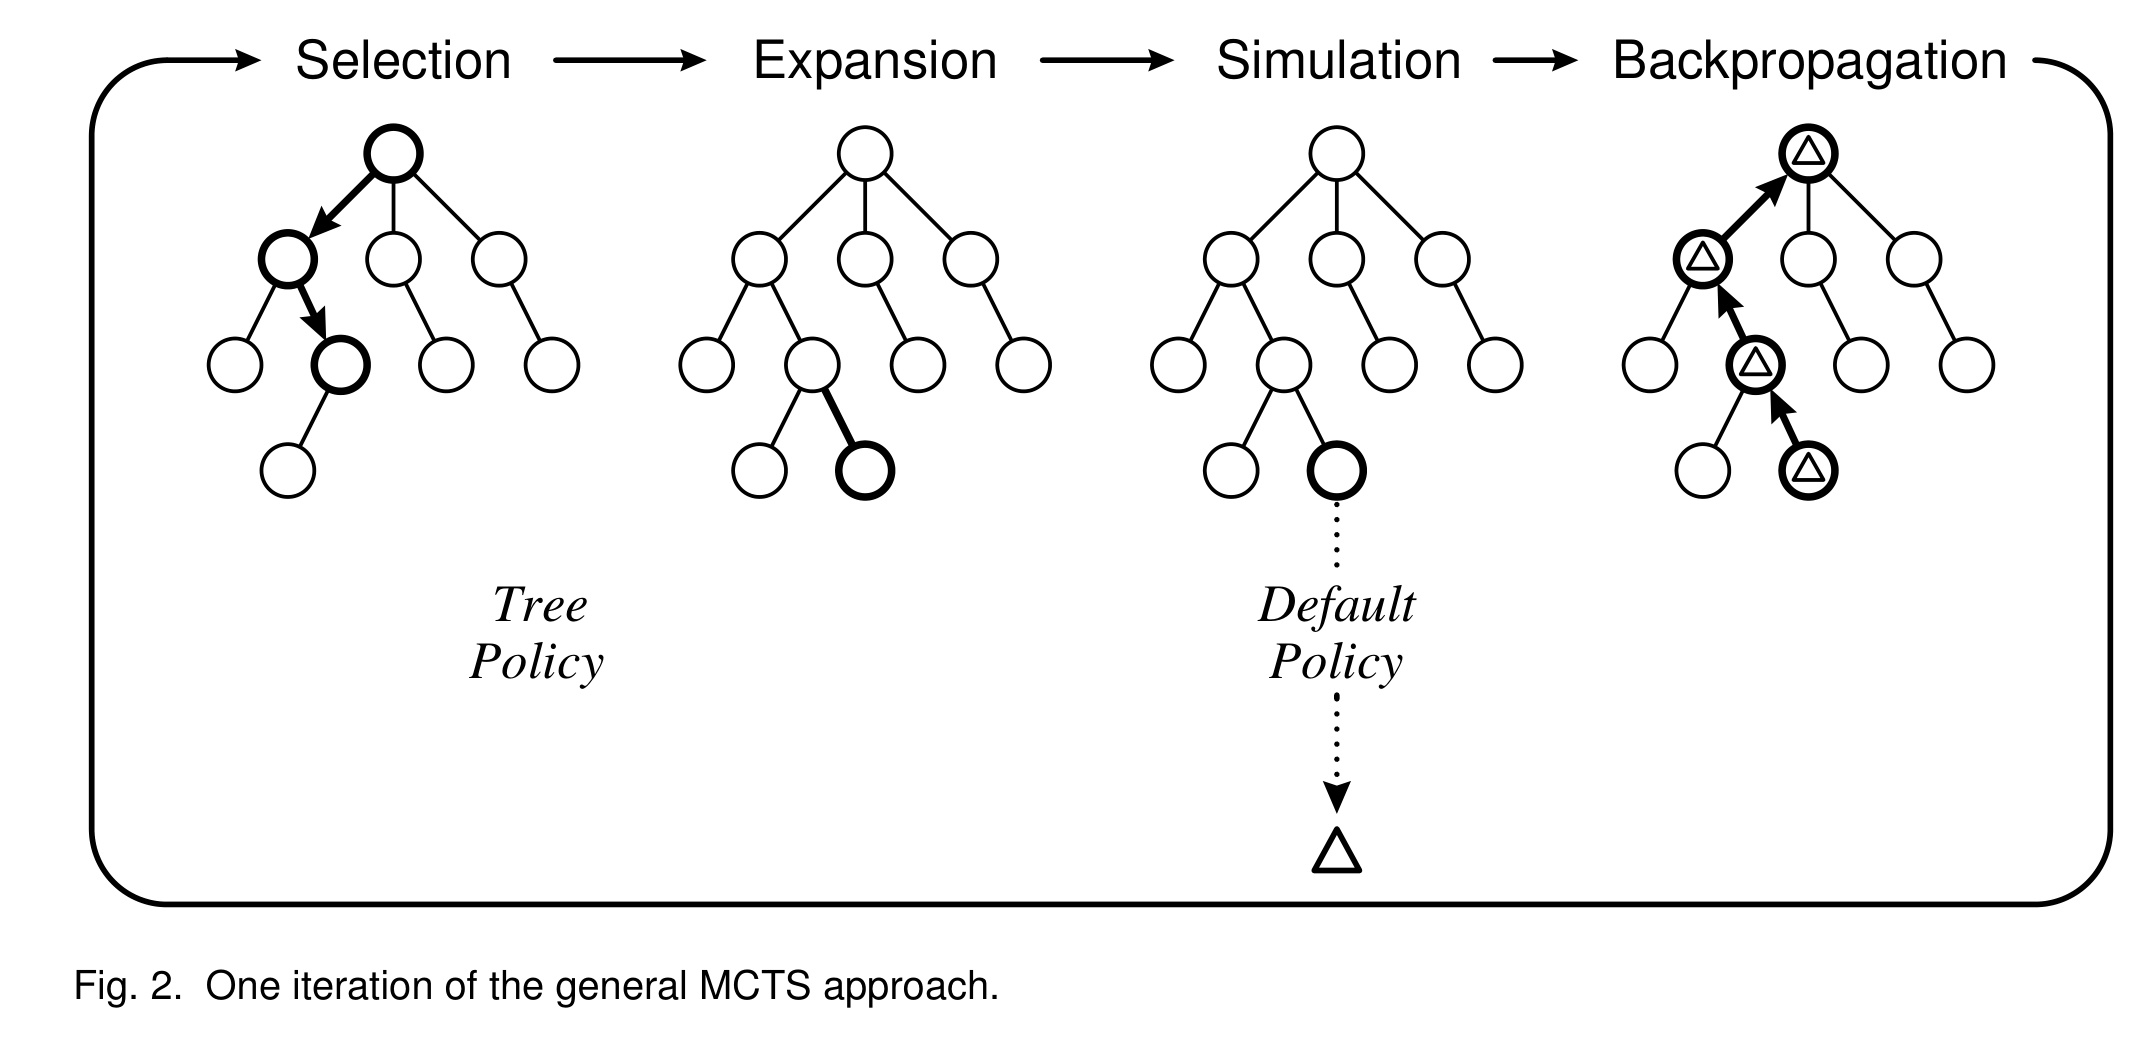
\includegraphics[height=7cm]{\rlroot/images/mcts_approach.jpg}
    \label{fig:mcts_approach}
\end{figure}

\end{enumerate}

上面描述的是UCT (UCB for Tree)算法,可以说是最经典的蒙特卡罗树搜索算法了。
但随着算法的发展,MCTS已经有了非常大的改变。
例如很多围棋AI都已经不再使用纯粹的UCB公式而改用效果更好的UCB1-Tuned了,而搜索方法上也有了非常多的改动了。

Reference:
\begin{itemize}
\item Browne C B, Powley E, Whitehouse D, et al. A Survey of Monte Carlo Tree Search Methods[J]. IEEE Transactions on Computational Intelligence \& Ai in Games, 2012, 4:1(1):1-43.
\item P. Auer, N. Cesa-Bianchi, and P. Fischer, “Finite-time Analysis  of the Multiarmed Bandit Problem,” Mach. Learn., vol. 47, no. 2,  pp. 235-256, 2002.
\end{itemize}

\section{GO}

\url{https://github.com/ardanlabs/gotraining}

\href{https://www.tastehit.com/blog/google-deepmind-alphago-how-it-works/}{Google DeepMind's AlphaGo: How it works}

\href{http://gopherdata.io/post/build_ml_powered_game_ai_tensorflow/}{Building an ML-Powered Game AI using TensorFlow in Go}

\href{https://github.com/TheDuck314/go-NN}{Go-playing neural network in Python using TensorFlow}

\begin{itemize}
\item \href{https://arxiv.org/pdf/1704.03732.pdf}{Learning from Demonstrations for Real World Reinforcement Learning}
\item \href{https://arxiv.org/abs/1312.5602}{Playing Atari with Deep Reinforcement Learning}
\item \href{https://www.intelnervana.com/demystifying-deep-reinforcement-learning/}{Guest Post (Part I): Demystifying Deep Reinforcement Learning}
\item \href{https://storage.googleapis.com/deepmind-media/dqn/DQNNaturePaper.pdf}{Human-level control through deep reinforcement learning}
\item \href{http://simplecore-dev.intel.com/nervana/wp-content/uploads/sites/55/2015/12/ProofQlearning.pdf}{Convergence of Q-learning: a simple proof}
\end{itemize}

$<s, a, r, s'>$

\subsection{贝尔曼方程(Bellman Equation)}
\href{https://zhuanlan.zhihu.com/p/21340755?refer=intelligentunit}{DQN 从入门到放弃3 价值函数与Bellman方程}

\subsection{bandit老虎机}
多臂老虎机

\ifx\mlnotes\undefined
    \bibliography{\notesroot/reference/reference.bib}
\end{document}

\fi


\ifx\notes\undefined
    \bibliography{\notesroot/reference/reference.bib}
\end{document}

\fi
